\documentclass[a4paper]{report}

\usepackage[latte]{catppuccinpalette}

\usepackage{amsmath}
\usepackage{amsthm}
\theoremstyle{definition}
\newtheorem{definition}{\textcolor{CtpLatteBlue}{Definition}}[section]
\theoremstyle{plain}
\newtheorem{theorem}{\textcolor{CtpLatteRed}{Theorem}}[section]
\newtheorem{proposition}{\textcolor{CtpLatteMaroon}{Proposition}}[section]
\theoremstyle{remark}
\newtheorem*{remark}{\textcolor{CtpLatteYellow}{Remark}}
\newtheorem{example}{\textcolor{CtpLatteGreen}{Example}}[section]
\newenvironment{solution}{\begin{proof}[Solution]}{\end{proof}}

\usepackage{newpx}

\usepackage{imakeidx}
\makeindex[options=-s main.ist]
\usepackage{pgfplots}
\pgfplotsset{compat=1.18}
\usepackage{booktabs}
\usepackage[hidelinks,pdftitle={Notes on Probability Theory and Stochastic Processes},pdfauthor={Henry Tan}]{hyperref}

\title{Notes on Probability Theory \\and Stochastic Processes}
\author{Henry Tan}
\date{Spring Semester, 2026}

\begin{document}

\sloppy

\pagenumbering{gobble}

\maketitle

\pagestyle{headings}

\pagenumbering{roman}

\cleardoublepage
\phantomsection
\addcontentsline{toc}{chapter}{Preface}
\chapter*{Preface}

Probability theory studies the mathematical framework for quantifying random events and their likelihoods, while stochastic processes extend this framework to model systems that evolve randomly over time. The core concepts of this field are crucial for understanding phenomena encountered in engineering, such as communication systems, signal processing, and machine learning.

This notebook includes the necessary definitions, theorems, and examples for the 3412110099 (or BBC4941) Probability Theory and Stochastic Processes module, which I am taking in the spring semester of 2026 as part of the Joint Programme between Beijing University of Posts and Telecommunications (BUPT) and Queen Mary University of London (QMUL). Most of the content is based on the lecture slides provided by Professor YANG Jiankui at BUPT. GenAI tools have been used to assist in writing some of the solutions and explanations.

This notebook comprises nine chapters and an index, structured as follows:
\begin{description}
  \item[Chapter 0] reviews some basic concepts in calculus and complex analysis, which are necessary for understanding the content in the following chapters.
  \item[Chapter 1] gives the definition of probability and some of its properties, and introduces the concept of conditional probability and independence, which are fundamental for understanding how events relate to each other.
  \item[Chapter 2] defines random variables, distributions, and their numerical characteristics. Some common discrete and continuous distributions are also introduced, which are widely used in modeling random phenomena.
  \item[Chapter 3] extends the concept of random variables to random vectors, and introduces the joint distribution, marginal distribution, and conditional distribution of random vectors. The covariance matrix and correlation coefficient are also defined, which are important for understanding the relationships between different random variables.
  \item[Chapter 4] presents some limit theorems, which are fundamental results in probability theory that describe the behavior of sums of random variables.
  \item[Chapter 5] introduces stochastic processes by defining them and discussing their properties and classifications.
  \item[Chapter 6] focuses on stationary stochastic processes, which are a special class of stochastic processes that have statistical properties that do not change over time. The power spectral density is also introduced.
  \item[Chapter 7] introduces discrete-time Markov chains, which are a type of stochastic process that has the Markov property, meaning that the future state depends only on the current state and not on the past states.
  \item[Chapter 8] introduces independent increment processes, along with the Poisson process, Gaussian process, Brownian motion, and Wiener process, which are important examples of stochastic processes with independent increments.
  \item[Index] serves as a quick reference for the key terms and theorems.
\end{description}
Please note that Chapter 4 and the following chapters are still under construction and review, and will be updated in the future.

I hope this notebook can be a useful resource for students taking this module, and I welcome any feedback or suggestions for improvement. Let's enjoy the journey of learning probability theory and stochastic processes together! (\^{}~--~\^{})/'

\vspace{2em}
\begin{flushright}
  Henry Tan\\
  \href{https://github.com/Henry0512}{https://github.com/Henry0512}\\
  \today
\end{flushright}

\cleardoublepage
\phantomsection
\addcontentsline{toc}{chapter}{Contents}
\tableofcontents

\cleardoublepage

\pagenumbering{arabic}

\setcounter{chapter}{-1}
\chapter{Calculus Basics}

\section{Limits and Series}

\begin{theorem}[Important Limits]
  The following limits are fundamental in calculus and analysis:
  \begin{enumerate}
    \item $\displaystyle \lim_{n \to \infty} \left(1 + \frac{x}{n}\right)^n = e^x$, for any $x \in \mathbb{R}$.
    \item $\displaystyle \lim_{x \to 0} \frac{\sin x}{x} = 1$.
  \end{enumerate}
\end{theorem}

\begin{theorem}[Taylor Series]\index{Taylor series}
  The Taylor series expansion of some common functions are:
  \begin{enumerate}
    \item Exponential function: $\displaystyle e^x = \sum_{n=0}^\infty \frac{x^n}{n!} = 1 + x + \frac{x^2}{2!} + \frac{x^3}{3!} + \cdots$
    \item Geometric series: For $|x| < 1$, $\displaystyle \frac{1}{1-x} = \sum_{n=0}^\infty x^n = 1 + x + x^2 + \cdots$
    \item Logarithmic function: For $-1 < x \le 1$, $\displaystyle \ln(1+x) = \sum_{n=1}^\infty \frac{(-1)^{n-1} x^n}{n} = x - \frac{x^2}{2} + \frac{x^3}{3} - \cdots$
  \end{enumerate}
\end{theorem}

\section{Integration Techniques}

\begin{theorem}[Integration by Parts]\index{integration by parts}
  Let $u$ and $v$ be differentiable functions. Then
  \[
    \int u\,\mathrm{d}v = u v - \int v\,\mathrm{d}u.
  \]
\end{theorem}

\begin{theorem}[Substitution Rule]\index{substitution rule}
  If $x = g(t)$ is a continuously differentiable function, and $f$ is continuous on the range of $g$, then for indefinite integrals:
  \[
    \int f(x)\,\mathrm{d}x = \int f(g(t)) g'(t)\,\mathrm{d}t.
  \]
  For definite integrals, this becomes:
  \[
    \int_{g(c)}^{g(d)} f(x)\,\mathrm{d}x = \int_c^d f(g(t)) g'(t)\,\mathrm{d}t.
  \]
\end{theorem}

\begin{theorem}[Fundamental Theorem of Calculus]\index{fundamental theorem of calculus}
  If $f$ is continuous on $[a,b]$ and $F$ is an antiderivative of $f$ on $[a,b]$, then
  \[
    \int_a^b f(x)\,\mathrm{d}x = F(b) - F(a).
  \]
\end{theorem}

\begin{theorem}[Leibniz Integral Rule]\index{Leibniz integral rule}\index{variable limits}
  For a definite integral with variable limits $a(x)$ and $b(x)$, the derivative with respect to $x$ is given by:
  \[
    \frac{\mathrm{d}}{\mathrm{d}x} \int_{a(x)}^{b(x)} f(t)\,\mathrm{d}t = f(b(x)) b'(x) - f(a(x)) a'(x).
  \]
  More generally, if the integrand also depends on $x$, i.e., $f(x, t)$, and both $f$ and $\frac{\partial f}{\partial x}$ are continuous:
  \[
    \frac{\mathrm{d}}{\mathrm{d}x} \int_{a(x)}^{b(x)} f(x, t)\,\mathrm{d}t = f(x, b(x)) b'(x) - f(x, a(x)) a'(x) + \int_{a(x)}^{b(x)} \frac{\partial f}{\partial x}(x, t)\,\mathrm{d}t.
  \]
\end{theorem}

\begin{theorem}[Important Integrals]\label{thm:important_integrals}
  The following integrals are commonly encountered in probability and statistics:
  \begin{enumerate}
    \item $\displaystyle \int_0^\infty e^{-ax^2}\,\mathrm{d}x = \frac{\sqrt{\pi}}{2\sqrt{a}}$, for $a > 0$.
    \item $\displaystyle \int_0^\infty x e^{-ax^2}\,\mathrm{d}x = \frac{1}{2a}$, for $a > 0$.
    \item $\displaystyle \int_0^\infty x^2 e^{-ax^2}\,\mathrm{d}x = \frac{\sqrt{\pi}}{4a^{3/2}}$, for $a > 0$.
    \item $\displaystyle \int_0^\infty x^n e^{-ax^2}\,\mathrm{d}x = \frac{1}{2} a^{-\frac{n+1}{2}} \Gamma\left(\frac{n+1}{2}\right)$, for $a > 0$ and $n \in \mathbb{N}$.
  \end{enumerate}
\end{theorem}

We can show the first integral using polar coordinates as follows:
\begin{proof}
  Let $I = \int_0^\infty e^{-ax^2}\,\mathrm{d}x$. Then
  \[
    I^2 = \left( \int_0^\infty e^{-ax^2}\,\mathrm{d}x \right) \left( \int_0^\infty e^{-ay^2}\,\mathrm{d}y \right) = \int_0^\infty \int_0^\infty e^{-a(x^2 + y^2)}\,\mathrm{d}x\,\mathrm{d}y.
  \]
  Converting to polar coordinates, where $x = r\cos\theta$ and $y = r\sin\theta$, we have $x^2 + y^2 = r^2$ and $\mathrm{d}x\,\mathrm{d}y = r\,\mathrm{d}r\,\mathrm{d}\theta$. The limits of integration for $r$ are from $0$ to $\infty$, and for $\theta$ are from $0$ to $\pi/2$. Thus,
  \[
    I^2 = \int_0^{\pi/2} \int_0^\infty e^{-ar^2} r\,\mathrm{d}r\,\mathrm{d}\theta.
  \]
  Evaluating the inner integral with respect to $r$, we use the substitution $u = ar^2$, which gives $\mathrm{d}u = 2ar\,\mathrm{d}r$. Therefore,
  \[
    \int_0^\infty e^{-ar^2} r\,\mathrm{d}r = \frac{1}{2a} \int_0^\infty e^{-u}\,\mathrm{d}u = \frac{1}{2a}.
  \]
  Now, integrating with respect to $\theta$,
  \[
    I^2 = \int_0^{\pi/2} \frac{1}{2a}\,\mathrm{d}\theta = \frac{\pi}{4a}.
  \]
  Taking the square root gives
  \[
    I = \sqrt{\frac{\pi}{4a}} = \frac{\sqrt{\pi}}{2\sqrt{a}}. \qedhere
  \]
\end{proof}

The second integral can be evaluated using a simple substitution:
\begin{proof}
  Let $u = ax^2$. Then $\mathrm{d}u = 2ax\,\mathrm{d}x$, or $x\,\mathrm{d}x = \frac{1}{2a}\,\mathrm{d}u$. The limits of integration remain $0$ to $\infty$. Substituting these into the integral gives
  \[
    \int_0^\infty x e^{-ax^2}\,\mathrm{d}x = \int_0^\infty e^{-u} \frac{1}{2a}\,\mathrm{d}u = \frac{1}{2a} \left[ -e^{-u} \right]_0^\infty = \frac{1}{2a} (0 - (-1)) = \frac{1}{2a}. \qedhere
  \]
\end{proof}

The third integral can be derived by differentiating the first integral with respect to $a$:
\begin{proof}
  Let $I(a) = \int_0^\infty e^{-ax^2}\,\mathrm{d}x = \frac{\sqrt{\pi}}{2} a^{-1/2}$. Differentiating both sides with respect to $a$ yields
  \[
    \frac{\mathrm{d}}{\mathrm{d}a} I(a) = \int_0^\infty \frac{\partial}{\partial a} \left( e^{-ax^2} \right)\,\mathrm{d}x = \int_0^\infty (-x^2) e^{-ax^2}\,\mathrm{d}x.
  \]
  On the other hand, differentiating the evaluated result gives
  \[
    \frac{\mathrm{d}}{\mathrm{d}a} \left( \frac{\sqrt{\pi}}{2} a^{-1/2} \right) = \frac{\sqrt{\pi}}{2} \left( -\frac{1}{2} \right) a^{-3/2} = -\frac{\sqrt{\pi}}{4a^{3/2}}.
  \]
  Equating the two expressions and multiplying by $-1$, we obtain
  \[
    \int_0^\infty x^2 e^{-ax^2}\,\mathrm{d}x = \frac{\sqrt{\pi}}{4a^{3/2}}. \qedhere
  \]
\end{proof}
This can also be derived using integration by parts:
\begin{proof}
  Let $u = x$ and $\mathrm{d}v = x e^{-ax^2}\,\mathrm{d}x$. Then $\mathrm{d}u = \mathrm{d}x$ and $v = -\frac{1}{2a} e^{-ax^2}$. Applying integration by parts gives
  \[
    \int_0^\infty x^2 e^{-ax^2}\,\mathrm{d}x = uv \bigg|_0^\infty - \int_0^\infty v\,\mathrm{d}u = \left[ -\frac{x}{2a} e^{-ax^2} \right]_0^\infty + \frac{1}{2a} \int_0^\infty e^{-ax^2}\,\mathrm{d}x.
  \]
  The limit \(\lim_{x \to \infty} -\frac{x}{2a} e^{-ax^2} = 0\), and the remaining integral is the first integral we evaluated. Thus,
  \[
    \int_0^\infty x^2 e^{-ax^2}\,\mathrm{d}x = \frac{1}{2a} \cdot \frac{\sqrt{\pi}}{2\sqrt{a}} = \frac{\sqrt{\pi}}{4a^{3/2}}. \qedhere
  \]
\end{proof}

For the higher-order integral, we can use the substitution $u = ax^2$ again:
\begin{proof}
  Let $u = ax^2$, then $x = \left(\frac{u}{a}\right)^{1/2}$ and $\mathrm{d}x = \frac{1}{2\sqrt{a}} u^{-1/2}\,\mathrm{d}u$. The limits of integration remain $0$ to $\infty$. Substituting these into the integral gives
  \[
    \int_0^\infty x^n e^{-ax^2}\,\mathrm{d}x = \int_0^\infty \left(\frac{u}{a}\right)^{n/2} e^{-u} \frac{1}{2\sqrt{a}} u^{-1/2}\,\mathrm{d}u = \frac{1}{2} a^{-\frac{n+1}{2}} \int_0^\infty u^{\frac{n-1}{2}} e^{-u}\,\mathrm{d}u.
  \]
  The remaining integral is the Gamma function evaluated at $\frac{n+1}{2}$, so we have
  \[
    \int_0^\infty x^n e^{-ax^2}\,\mathrm{d}x = \frac{1}{2} a^{-\frac{n+1}{2}} \Gamma\left( \frac{n+1}{2} \right). \qedhere
  \]
\end{proof}

\section{Multivariate Calculus}

\begin{definition}[Double Integral]\index{double integral}
  The \emph{double integral} of a function $f(x, y)$ over a region $R$ in the $xy$-plane is defined as
  \[
    \iint_R f(x, y)\,\mathrm{d}x\,\mathrm{d}y = \lim_{m, n \to \infty} \sum_{i=1}^m \sum_{j=1}^n f(x_{ij}, y_{ij}) \Delta x \Delta y,
  \]
  where $R$ is partitioned into $m$ subintervals in the $x$-direction and $n$ subintervals in the $y$-direction, and $(x_{ij}, y_{ij})$ is a sample point in the $(i,j)$-th subrectangle.
\end{definition}

\begin{theorem}[Fubini's Theorem]\index{Fubini's theorem}
  If $f(x, y)$ is continuous on a rectangular region $R = [a, b] \times [c, d]$, then
  \[
    \iint_R f(x, y)\,\mathrm{d}x\,\mathrm{d}y = \int_a^b \left( \int_c^d f(x, y)\,\mathrm{d}y \right) \mathrm{d}x = \int_c^d \left( \int_a^b f(x, y)\,\mathrm{d}x \right) \mathrm{d}y.
  \]
\end{theorem}

\begin{theorem}[Double Integrals in Polar Coordinates]\index{polar coordinates}
  To evaluate a double integral over a region $R$ in the $xy$-plane using polar coordinates $(r, \theta)$, we use the transformation $x = r\cos\theta$ and $y = r\sin\theta$. The area element becomes $\mathrm{d}x\,\mathrm{d}y = r\,\mathrm{d}r\,\mathrm{d}\theta$. Then
  \[
    \iint_R f(x, y)\,\mathrm{d}x\,\mathrm{d}y = \iint_S f(r\cos\theta, r\sin\theta) r\,\mathrm{d}r\,\mathrm{d}\theta,
  \]
  where $S$ is the region in the $r\theta$-plane corresponding to $R$.
\end{theorem}

\begin{definition}[Jacobian]\index{Jacobian}
  Let $x = g(u, v)$ and $y = h(u, v)$ be a transformation. The \emph{Jacobian} of this transformation is given by the determinant
  \[
    J(u, v) = \frac{\partial(x, y)}{\partial(u, v)} = \det \begin{pmatrix}
      \frac{\partial x}{\partial u} & \frac{\partial x}{\partial v} \\
      \frac{\partial y}{\partial u} & \frac{\partial y}{\partial v}
    \end{pmatrix}.
  \]
  The transformation of double integrals is then
  \[
    \iint_R f(x, y)\,\mathrm{d}x\,\mathrm{d}y = \iint_S f(g(u, v), h(u, v)) |J(u, v)|\,\mathrm{d}u\,\mathrm{d}v.
  \]
\end{definition}

\section{Special Functions}

\begin{definition}[Gamma Function]\index{Gamma function}
  The \emph{Gamma function}, denoted by $\Gamma(z)$, is an extension of the factorial function to complex (and real) numbers. For $z > 0$, it is defined by the integral
  \[
    \Gamma(z) = \int_0^\infty t^{z-1} e^{-t}\,\mathrm{d}t.
  \]
\end{definition}

\begin{proposition}
  The Gamma function has the following properties:
  \begin{enumerate}
    \item $\Gamma(z+1) = z \Gamma(z)$ for any $z > 0$.
    \item If $n$ is a positive integer, $\Gamma(n) = (n-1)!$.
    \item $\Gamma(1/2) = \sqrt{\pi}$.
  \end{enumerate}
\end{proposition}

\begin{definition}[Beta Function]\index{Beta function}
  The \emph{Beta function}, denoted by $\mathrm{B}(x, y)$, is defined for $x, y > 0$ by the integral
  \[
    \mathrm{B}(x, y) = \int_0^1 t^{x-1} (1-t)^{y-1}\,\mathrm{d}t.
  \]
\end{definition}

\begin{proposition}
  The Beta function is related to the Gamma function by
  \[
    \mathrm{B}(x, y) = \frac{\Gamma(x)\Gamma(y)}{\Gamma(x+y)}.
  \]
\end{proposition}

\chapter{Events and Their Probabilities}

\section{Experiment, Sample Space, and Random Event}

\begin{definition}[Sample Space]\index{sample space}
  The set for all possible outcomes of an random experiment (if we could know all possible outcomes) is known as the \emph{sample space}.
\end{definition}

\begin{definition}[Random Event]\index{random event}\index{event}
  Any subset of the sample space \(S\) (or \(\Omega\)) is known as an \emph{random event} or \emph{event}.
\end{definition}
Events are usually denoted by capital letters.

\begin{itemize}
  \index{inevitable event}\index{impossible event}
  \item Inevitable event: \(S\) or \(\Omega\)
  \item Impossible event: \(\varnothing\)
\end{itemize}
\begin{remark}
An event with probability 0 is not necessarily an impossible event, and an event with probability 1 is not necessarily an inevitable event.
\end{remark}
\begin{example}
  Consider generating a random number \(X\) uniformly distributed on the interval \([0, 1]\). The event \(A = \{X = 0.5\}\) has probability 0, but it is not an impossible event since it can occur.
\end{example}

Some events can be expressed in terms of other events. For example, if \(A\) and \(B\) are two events, then we can define the following events:
\begin{enumerate}
  \index{subset}\index{union}\index{intersection}\index{set difference}\index{disjoint events}\index{complement}
  \item \(A \subset B\) means if event \(A\) occurs, then event \(B\) also occurs.
  \item \(A = B\) means \(A \subset B\) and \(B \subset A\), i.e., \(A\) and \(B\) are the same event.
  \item \(A \cup B\) occurs if either event \(A\) or event \(B\) (or both) occur.
  \item \(A B\) or \(A \cap B\) occurs if both event \(A\) and event \(B\) occur.
  \item \(A \setminus B\) occurs if event \(A\) occurs but event \(B\) does not occur.
  \item \(A B = \varnothing\) means events \(A\) and \(B\) are \emph{disjoint} or \emph{mutually exclusive}, i.e., they cannot occur at the same time.
  \item \(A^c\) or \(\overline{A}\) is the \emph{complement} of event \(A\), \(A \cup \overline{A} = \Omega\) and \(A \overline{A} = \varnothing\).
\end{enumerate}

\begin{example}
  Select points randomly from unit circle. Let
  \[
  A_n = \left\{(x,y) \vert x^2 + y^2 < \frac{1}{n^2}\right\}, n = 1, 2, \dots
  \]
  then
  \[
    \bigcap_{n=1}^\infty A_n = \{(0, 0)\},
  \]
  but
  \[
    \bigcup_{n=1}^\infty A_n = \left\{(x,y) \vert x^2 + y^2 < 1\right\}.
  \]
\end{example}

\begin{proposition}
  Let \(A\), \(B\) and \(C\) be the random events. Then we have the following properties:
  \begin{enumerate}\index{De Morgan's Laws}
    \item Commutativity: \(A \cup B = B \cup A\), \(A B = B A\)
    \item Associativity: \(A \cup (B \cup C) = (A \cup B) \cup C = A \cup B \cup C\), \(A (B C) = (A B) C = A B C\)
    \item Distributivity: \(A (B \cup C) = A B \cup A C\), \(A \cup (B C) = (A \cup B)(A \cup C)\)
    \item De Morgan's Laws: \((A \cup B)^c = \overline{A} \cap \overline{B}\), \((A \cap B)^c = \overline{A} \cup \overline{B}\), \(\left(\bigcup_{i=1}^n A_i\right)^c = \bigcap_{i=1}^n \overline{A}_i\), \(\left(\bigcap_{i=1}^n A_i\right)^c = \bigcup_{i=1}^n \overline{A}_i\)
    \item \(A \cup B = A \cup \overline{A} B\), \(A \cup B \cup C = A \cup \overline{A} B \cup \overline{A} \overline{B} C\)
  \end{enumerate}
\end{proposition}

\section{Probabilities of Defined on Events}

\begin{definition}[Classical Random Experiment]\index{classical random experiment}\index{simple space}
  A random experiment \(E\) is \emph{classical} if
  \begin{enumerate}
    \item \(E\) contains only different finite sample points, i.e., \(\Omega = \{\omega_1, \omega_2, \dots, \omega_n\}\). We call this kind of sample space \emph{simple space}.
    \item All outcomes are equally likely to occur.
  \end{enumerate}
\end{definition}

If \(A\) is comprised by \(k\) different elementary events, then
\[
  P(A) = \frac{k}{n}.
\]

\begin{definition}[Geometric Random Experiment]\index{geometric random experiment}
  A random experiment \(E\) is \emph{geometric} if
  \begin{enumerate}
    \item The sample space is measurable (such as length, area, volume, etc.) region, i.e., \(0 < \mathrm{L}(\Omega) < \infty\).
    \item The probability of every event \(A \subseteq \Omega\) is proportional to the measure \(L(A)\) and has nothing to do with its position and shape.
  \end{enumerate}
\end{definition}

In a geometric random experiment, the probability of an event \(A\) is given by
\[
  P(A) = \frac{\mathrm{L}(A)}{\mathrm{L}(\Omega)}.
\]

Bertrand's paradox is a famous problem in geometric probability, which shows that the probability of an event can depend on the method of random selection, even if the underlying geometric conditions are the same.

\begin{definition}[Relative Frequency]\index{relative frequency}
  Let \(E\) be an random experiment, \(A\) be an ramdom event. Suppose that \(E\) was repeated \(n\) times under similiar conditions. Let \(f_n(A)\) be the times that \(A\) occurs. The ratio \(\frac{f_n(A)}{n}\) is called the \emph{relative frequency} of event \(A\) in \(n\) trials.
\end{definition}

\begin{theorem}
  For classical random experiment \(E\), the probability has the following properties:
  \begin{enumerate}
    \item for every event \(A\), \(P(A) \geq 0\);
    \item \(P(\Omega) = 1\);
    \item (finite additivity) for every sequence of disjoint events \(A_1, A_2, \dots, A_m\), we have
    \[
      P\left(\bigcup_{i=1}^m A_i\right) = \sum_{i=1}^m P(A_i), \quad m = 1, 2, \dots, n.
    \]
  \end{enumerate}
\end{theorem}

\begin{theorem}
  For geometric random experiment \(E\), the probability has the following properties:
  \begin{enumerate}
    \item for every event \(A\), \(P(A) \geq 0\);
    \item \(P(\Omega) = 1\);
    \item (countable additivity) for every sequence of disjoint events \(A_1, A_2, \dots\), we have
    \[
      P\left(\bigcup_{i=1}^\infty A_i\right) = \sum_{i=1}^\infty P(A_i).
    \]
  \end{enumerate}
\end{theorem}

\begin{theorem}
  For a random experiment \(E\), the frequency has the following properties:
  \begin{enumerate}
    \item for every event \(A\), \(F_n(A) \geq 0\);
    \item \(F_n(\Omega) = 1\);
    \item (finite additivity) for every sequence of disjoint events \(A_1, A_2, \dots, A_m\),
    \[
      F_n\left(\bigcup_{i=1}^m A_i\right) = \sum_{i=1}^m F_n(A_i), \quad m = 1, 2, \dots, n.
    \]
  \end{enumerate}
\end{theorem}

\begin{definition}[\(\sigma\)-algebra]\index{\(\sigma\)-algebra}
  A collection \(\mathcal{F}\) of subsets of \(\Omega\) is a \emph{\(\sigma\)-algebra} if
  \begin{enumerate}
    \item \(\Omega \in \mathcal{F}\);
    \item if \(A \in \mathcal{F}\), then \(\overline{A} \in \mathcal{F}\);
    \item if \(A_n \in \mathcal{F}\) for \(n = 1, 2, \dots\), then \(\bigcup_{n=1}^\infty A_n \in \mathcal{F}\).
  \end{enumerate}
\end{definition}

That is, a \(\sigma\)-algebra is a collection of subsets of \(\Omega\) that contains \(\Omega\) itself, is closed under complementation, and is closed under countable unions.

\begin{example}
  Let the experiment be a coin toss. Then \(\Omega = \{H, T\}\). Let \(\mathcal{F}_1 = \{\varnothing, \{H\}, \{T\}, \Omega\}\) and \(\mathcal{F}_2 = \{\varnothing, \Omega\}\). Then both \(\mathcal{F}_1\) and \(\mathcal{F}_2\) are \(\sigma\)-algebras on \(\Omega\).
\end{example}

\begin{proposition}
  If \(\mathcal{F}\) is a \(\sigma\)-algebra on \(\Omega\), then it has the following properties:
  \begin{enumerate}
    \item \(\varnothing \in \mathcal{F}\);
    \item if \(A, B \in \mathcal{F}\), then \(A B \in \mathcal{F}\) and \(A \setminus B \in \mathcal{F}\);
    \item if \(A_i \in \mathcal{F} (i = 1, 2, \dots, n)\), then \(\bigcup_{i=1}^n A_i \in \mathcal{F}\) and \(\bigcap_{i=1}^n A_i \in \mathcal{F}\);
    \item if \(A_i \in \mathcal{F} (i = 1, 2, \dots)\), then \(\bigcap_{i=1}^\infty A_i \in \mathcal{F}\).
  \end{enumerate}
\end{proposition}

\section{Axiomatic Definition of Probability}

\begin{definition}[Probability]\index{probability}\index{probability space}
  Let \(P(A) (A \in \mathcal{F})\) be a non-negative set function on the \(\sigma\)-algebra \(\mathcal{F}\). Then \(P(A)\) is called the \emph{probability of event \(A\)} if it satisfies the following axioms:
  \begin{enumerate}
    \item \(P(A) \geq 0\) for every event \(A \in \mathcal{F}\);
    \item \(P(\Omega) = 1\);
    \item (countable additivity) for every infinite sequence of countably disjoint events \(A_1, A_2, \dots\), we have
    \[
      P\left(\bigcup_{i=1}^\infty A_i\right) = \sum_{i=1}^\infty P(A_i).
    \]
  \end{enumerate}
  The sets in \(\mathcal{F}\) are called \emph{events}, and \(\mathcal{F}\) is called the \emph{algebra of events}. The triple \((\Omega, \mathcal{F}, P)\) is called a \emph{probability space} or \emph{probability triplet}.
\end{definition}

\begin{proposition}
  Some properties of probability can be derived from the axioms:
  \begin{enumerate}
    \item \(P(\varnothing) = 0\);
    \item for every finite sequence of disjoint events \(A_1, A_2, \dots, A_n\), we have
    \[
      P\left(\bigcup_{i=1}^n A_i\right) = \sum_{i=1}^n P(A_i),
    \]
    \item \(P(A) = 1 - P(\overline{A})\);
    \item if \(A \subseteq B\), then \(P(B \setminus A) = P(B) - P(A)\) and \(P(A) \leq P(B)\);
    \item \(P(A \cup B) = P(A) + P(B) - P(A B)\), similarly, for every finite sequence of events \(A_1, A_2, \dots, A_n\), we have
    \[
      P\left(\bigcup_{i=1}^n A_i\right) = \sum_{i=1}^n P(A_i) - \sum_{1 \leq i < j \leq n} P(A_i A_j) + \dots + (-1)^{n-1} P\left(\bigcap_{i=1}^n A_i\right),
    \]
    \item Continuity: If \(A_n \uparrow A\) (i.e., \(A_1 \subseteq A_2 \subseteq \cdots\) and \(A = \bigcup_{n=1}^\infty A_n\)), then \(P(A) = \lim_{n \to \infty} P(A_n)\); if \(A_n \downarrow A\) (i.e., \(A_1 \supseteq A_2 \supseteq \cdots\) and \(A = \bigcap_{n=1}^\infty A_n\)), then \(P(A) = \lim_{n \to \infty} P(A_n)\).
  \end{enumerate}
\end{proposition}

\begin{proof}
  We only prove the continuity property for \(A_n \uparrow A\), the other case can be proved similarly.
  If \(A_n \uparrow A\), then
  \[
  A = \bigcup_{n=1}^\infty A_n = A_1 \cup A_2 \overline{A}_1 \cup A_3 \overline{A}_2 \cup \cdots,
  \]
  and
  \[
  A_1 \cup A_2 \overline{A}_1 \cup A_3 \overline{A}_2 \cup \dots \cup A_n \overline{A}_{n-1} = A_n.
  \]
  Let \(B_1 = A_1\) and \(B_n = A_n \overline{A}_{n-1}\) for \(n \geq 2\). Then
  \begin{align*}
    P(A) & = P\left(\bigcup_{n=1}^\infty B_n\right) = \sum_{n=1}^\infty P(B_n) = \lim_{n \to \infty} \sum_{i=1}^n P(B_i) \\
         & = \lim_{n \to \infty} P \left(\bigcup_{i=1}^n B_i\right) = \lim_{n \to \infty} P(A_n). \qedhere
  \end{align*}
\end{proof}

\section{Conditional Probability}

\begin{definition}[Conditional Probability]\index{conditional probability}
  Given two events \(A\) and \(B\) with \(P(B) > 0\), the \emph{conditional probability} of \(A\) given \(B\) is defined as
  \[
    P(A \vert B) = \frac{P(A B)}{P(B)}.
  \]
\end{definition}

\begin{theorem}
  If \(P(B) > 0\), then the conditional probability is also a probability, that is,
  \begin{enumerate}
    \item for every event \(A\), \(P(A \vert B) \geq 0\);
    \item \(P(\Omega \vert B) = 1\);
    \item for every infinite sequence of countably disjoint events \(A_1, A_2, \dots\), we have
    \[
      P\left(\bigcup_{i=1}^\infty A_i \vert B\right) = \sum_{i=1}^\infty P(A_i \vert B).
    \]
  \end{enumerate}
\end{theorem}

\begin{proposition}
  Some properties of conditional probability can be derived from the axioms:
  \begin{enumerate}
    \item \(P(\varnothing \vert B) = 0\);
    \item for every finite sequence of disjoint events \(A_1, A_2, \dots, A_n\), we have
    \[
      P\left(\bigcup_{i=1}^n A_i \vert B\right) = \sum_{i=1}^n P(A_i \vert B),
    \]
    \item \(P(A \vert B) = 1 - P(\overline{A} \vert B)\);
    \item if \(A \subseteq C\), then \(P(C \setminus A \vert B) = P(C \vert B) - P(A \vert B)\) and \(P(A \vert B) \leq P(C \vert B)\);
    \item \(P(A \cup C \vert B) = P(A \vert B) + P(C \vert B) - P(A C \vert B)\).
  \end{enumerate}
\end{proposition}

\begin{theorem}
  Assume that \(P(B) > 0\). Then
  \[
    P(A B) = P(B) P(A \vert B).
  \]
\end{theorem}

\begin{theorem}
  Suppose that \(A_1, A_2, \dots, A_n\) are events with \(P\left(\bigcap_{i=1}^{n-1} A_i\right) > 0\). Then
  \[
    P\left(\bigcap_{i=1}^n A_i\right) = P(A_1) P(A_2 \vert A_1) P(A_3 \vert A_1 A_2) \cdots P\left(A_n \vert \bigcap_{i=1}^{n-1} A_i\right).
  \]
\end{theorem}

\begin{example}
  Suppose that an urn box contains $r$ red balls and $b$ black balls ($r, b \geq 2$). We randomly select 1 ball from the box, and then put it back along with $c$ balls of the same color into the box. Then we randomly select another ball from the box. Determine the probability of obtaining the sequence of colors \texttt{red-red-black-black}.
\end{example}

\begin{solution}
  Let \(R_i\) be the event that the \(i\)-th selected ball is red, and let \(B_i\) be the event that the \(i\)-th selected ball is black. Then
  \begin{align*}
    P(R_1 R_2 B_3 B_4) & = P(R_1) P(R_2 \vert R_1) P(B_3 \vert R_1 R_2) P(B_4 \vert R_1 R_2 B_3) \\
                       & = \frac{r}{r + b} \cdot \frac{r + c}{r + b + c} \cdot \frac{b}{r + b + 2c} \cdot \frac{b + c}{r + b + 3c}. \qedhere
  \end{align*}
\end{solution}

\begin{theorem}[Total Probability Theorem]\index{total probability theorem}
  Suppose that \(B_1, B_2, \dots, B_n\) form a partition of the sample space \(\Omega\), and \(P(B_i) > 0\) for \(i = 1, 2, \dots, n\). Then
  \[
    P(A) = \sum_{i=1}^n P(B_i) P(A \vert B_i).
  \]
\end{theorem}

\begin{theorem}[Bayes' Theorem]\index{Bayes' theorem}
  Suppose that \(B_1, B_2, \dots, B_n\) form a partition of the sample space \(\Omega\), and \(P(B_i) > 0\) for \(i = 1, 2, \dots, n\). Let \(A\) be an event with \(P(A) > 0\). Then for every \(i = 1, 2, \dots, n\), we have
  \[
    P(B_i \vert A) = \frac{P(B_i) P(A \vert B_i)}{\sum_{j=1}^n P(B_j) P(A \vert B_j)}.
  \]
\end{theorem}

Bayes' Theorem can be rewritten as
\[
  \underbrace{P(C \vert A)}_{\text{posterior probability}} = \frac{\overbrace{P(C)}^{\text{prior probability}} \overbrace{P(A \vert C)}^{\text{conditional likelihood}}}{\underbrace{P(A)}_{\text{marginal likelihood}}}.
\]

\section{Independence of Events}

\begin{definition}[Independence]\index{independent events}
  Two events \(A\) and \(B\) are \emph{independent} if \(P(A B) = P(A) P(B)\).
\end{definition}

If \(P(B) > 0\), then \(A\) and \(B\) are independent if and only if \(P(A \vert B) = P(A)\). That is, the occurrence of event \(B\) does not affect the probability of event \(A\).

\begin{theorem}
  If \(A\) and \(B\) are independent, then \(A\) and \(\overline{B}\) are independent, \(\overline{A}\) and \(B\) are independent, and \(\overline{A}\) and \(\overline{B}\) are independent.
\end{theorem}

\begin{proof}
  We only prove that \(A\) and \(\overline{B}\) are independent, the other cases can be proved similarly. Since \(A\) and \(B\) are independent, we have
  \[
    P(A \overline{B}) = P(A) - P(A B) = P(A) - P(A) P(B) = P(A)(1 - P(B)) = P(A) P(\overline{B}). \qedhere
  \]
\end{proof}

\begin{example}
  Suppose that \(P(A) = 1\) and \(B \in \mathcal{F}\), we want to determine whether \(A\) and \(B\) are independent. Since \(P(A) = 1\), we have
  \[
    0 \leq P(\overline{A} B) \leq P(\overline{A}) = 0,
  \]
  which implies \(P(\overline{A} B) = 0\).
  Therefore, \(P(A B) = P(B) - P(\overline{A} B) = P(B) = P(A) P(B)\), and \(A\) and \(B\) are independent.
\end{example}

\begin{definition}[Mutual Independence]\index{mutual independence}\index{pairwise independence}
  Three events \(A\), \(B\) and \(C\) are \emph{mutually independent} (or \emph{independent}) if
  \begin{align*}
    P(A B) & = P(A) P(B), \\
    P(A C) & = P(A) P(C), \\
    P(B C) & = P(B) P(C), \\
    P(A B C) & = P(A) P(B) P(C).
  \end{align*}
  Events \(A\), \(B\) and \(C\) are \emph{pairwise independent} if only the first three conditions hold.
\end{definition}

\begin{definition}[Mutual Independence]\index{mutual independence}
  Events \(A_1, A_2, \dots, A_n\) are \emph{independent} if for every subset \(\{i_1, i_2, \dots, i_k\} \subseteq \{1, 2, \dots, n\}\) with \(k \geq 2\), we have
  \[
    P\left(\bigcap_{j=1}^k A_{i_j}\right) = \prod_{j=1}^k P(A_{i_j}).
  \]
\end{definition}

\begin{theorem}
  Events \(A_1, A_2, \dots, A_n\) are independent if and only if for every subset \(\{i_1, i_2, \dots, i_k\} \subseteq \{1, 2, \dots, n\}\) with \(k \geq 2\), we have
  \[
    P\left(\bigcap_{j=1}^k A_{i_j}^*\right) = \prod_{j=1}^k P(A_{i_j}^*),
  \]
  where \(A_i^*\) denotes \(A_i\) or \(\overline{A}_i\) for \(i = 1, 2, \dots, n\).
\end{theorem}

If events \(A_1, A_2, \dots, A_n\) are independent, by De Morgan's Laws, we have
\[
  P\left(\bigcup_{i=1}^n A_i\right) = 1 - P\left(\bigcap_{i=1}^n \overline{A}_i\right) = 1 - \prod_{i=1}^n (1 - P(A_i)),
\]
and
\[
  P\left(\bigcup_{i=1}^n \overline{A}_i\right) = 1 - P\left(\bigcap_{i=1}^n A_i\right) = 1 - \prod_{i=1}^n P(A_i).
\]

\begin{definition}[Bernoulli Trial]\index{Bernoulli trial}\index{Bernoulli process}
  A Bernoulli trial is a random experiment with only two possible outcomes, usually denoted as "success" and "failure". The probability of success is denoted by \(p\) and the probability of failure is denoted by \(q = 1 - p\). A sequence of independent Bernoulli trials is called a Bernoulli process.
\end{definition}

\begin{theorem}
  The probability that the outcome of an experiment that consists of \(n\) Bernoulli trials contains exactly \(k\) successes is given by the binomial distribution:
  \[
    P(X = k) = \binom{n}{k} p^k q^{n-k}, \quad k = 0, 1, \dots, n.
  \]
\end{theorem}
\chapter{Random Variable}

\section{The Definition of a Random Variable}

\begin{definition}[Random Variable]\index{random variable}
  A \emph{random variable} (r.v.) is a function \(X: \Omega \to \mathbb{R}\) that assigns a real number to each outcome in the sample space \(\Omega\).
\end{definition}

\begin{remark}
  Let \((\Omega, \mathcal{F}, P)\) be a probability space. In measure-theoretic probability, a random variable is defined as a measurable function \(X: \Omega \to \mathbb{R}\), s.t. \(X^{-1}(B) = \{\omega \in \Omega : X(\omega) \in B\} \in \mathcal{F}\) for all \(B \in \mathcal{B}(\mathbb{R})\), where \(\mathcal{B}(\mathbb{R})\) is the Borel \(\sigma\)-algebra on \(\mathbb{R}\).
\end{remark}

\begin{definition}[Discrete Random Variable]\index{discrete random variable}
  A random variable \(X\) is said to be \emph{discrete} type if the number of values it can take is finite or countably infinite.
\end{definition}

\section{Discrete Random Variables}

\begin{definition}[Probability Mass Function]\index{probability mass function}
  For a discrete random variable \(X\), the \emph{probability (mass) function} (p.f.) is defined as
  \[
    p(x) = P(X = x), \quad x \in \mathbb{R}.
  \]
\end{definition}

\begin{proposition}
  The function \(p(x)\) satisfies the following properties:
  \begin{enumerate}
    \item \(p(x) \geq 0\) for all \(x \in \mathbb{R}\).
    \item \(\sum_{i = 1}^\infty p(x_i) = 1\), where \(\{x_i\}\) is the set of all possible values of \(X\).
  \end{enumerate}
\end{proposition}

\begin{example}
  Bob is shooting. Suppose that the probability of hitting the target is 0.1. Suppose that each shooting is independent. Let \(X\) be the number of hits in 5 shootings. What is the probability of the event that Bob hits the target at least four times, i.e., \(P\{X \geq 4\}\)?
\end{example}
\begin{solution}
  By Bernoulli trial, we have
  \[
    P\{X = k\} = \binom{5}{k} (0.1)^k (0.9)^{5-k}, \quad k = 0, 1, 2, 3, 4, 5.
  \]
  Therefore,
  \[
    P\{X \geq 4\} = P\{X = 4\} + P\{X = 5\} = 0.00045 + 0.00001 = 0.00046. \qedhere
  \]
\end{solution}

\begin{definition}[Bernoulli Distribution]\index{Bernoulli distribution}\index{two-point distribution}
  A discrete random variable \(X\) is said to have a \emph{Bernoulli distribution} (or \emph{two-point distribution}) with parameter \(p\) if its probability mass function is given by
  \[
    p(x) = \begin{cases}
      p, & x = 1, \\
      1 - p, & x = 0. \\
    \end{cases}
  \]
\end{definition}

\begin{definition}[Binomial Distribution]\index{binomial distribution}
  A discrete random variable \(X\) is said to have a \emph{binomial distribution} with parameters \(n\) and \(p (0 < p < 1)\) if its probability mass function is given by
  \[
    P(X = k) = \binom{n}{k} p^k (1 - p)^{n - k}, \quad k = 0, 1, 2, \dots, n.
  \]
  We denote this distribution by \(X \sim \mathrm{B}(n, p)\).
\end{definition}

\begin{proposition}
  Let \(X \sim \mathrm{B}(n, p)\). The probability mass function \(f(k) = P(X = k)\) is unimodal. The set of modes, denoted by \(\mathcal{K}^* = \arg\max_{k \in \{0, \dots, n\}} P(X = k)\), is determined as follows:
  \begin{enumerate}
    \item If \((n+1)p\) is not an integer, there is a unique mode \(k^* = \lfloor (n+1)p \rfloor\). The sequence \(P(X=k)\) strictly increases for \(k \le k^*\) and strictly decreases for \(k \ge k^*\).
    \item If \((n+1)p\) is an integer, there are two adjacent modes \(k_1^* = (n+1)p - 1\) and \(k_2^* = (n+1)p\). In this case, \(P(X=k)\) strictly increases for \(k \le k_1^*\), satisfies \(P(X=k_1^*) = P(X=k_2^*)\), and strictly decreases for \(k \ge k_2^*\).
  \end{enumerate}
\end{proposition}
\begin{proof}
  For \(k = 0, 1, \dots, n-1\), we have
  \[
    \frac{P(X = k + 1)}{P(X = k)} = \frac{\binom{n}{k + 1} p^{k + 1} (1 - p)^{n - k - 1}}{\binom{n}{k} p^k (1 - p)^{n - k}} = \frac{n - k}{k + 1} \cdot \frac{p}{1 - p}.
  \]
  Therefore, \(P(X = k + 1) > P(X = k)\) if and only if \(k < (n + 1)p - 1\), and \(P(X = k + 1) < P(X = k)\) if and only if \(k > (n + 1)p - 1\). The rest of the proof follows immediately. \qedhere
\end{proof}

\begin{theorem}[Poisson Limit Theorem]\index{Poisson limit theorem}
  Suppose that \(\lambda > 0\) is a constant and \(n\) is a positive integer. If \(\lim_{n \to \infty} np_n = \lambda\), then for any fixed \(k = 0, 1, 2, \dots\), we have
  \[
    \lim_{n \to \infty} \binom{n}{k} p^k (1 - p)^{n - k} = \frac{\lambda^k e^{-\lambda}}{k!}.
  \]
\end{theorem}

\begin{definition}[Poisson Distribution]\index{Poisson distribution}
  A discrete random variable \(X\) is said to have a \emph{Poisson distribution} with parameter \(\lambda > 0\) if its probability mass function is given by
  \[
    P(X = k) = \frac{\lambda^k e^{-\lambda}}{k!}, \quad k = 0, 1, 2, \dots.
  \]
  We denote this distribution by \(X \sim \mathrm{Poi}(\lambda)\).
\end{definition}

The sum of the probabilities of a Poisson distribution is
\[
  \sum_{k = 0}^\infty \frac{\lambda^k e^{-\lambda}}{k!} = e^{-\lambda} \sum_{k = 0}^\infty \frac{\lambda^k}{k!} = e^{-\lambda} e^{\lambda} = 1.
\]

\begin{definition}[Geometric Distribution]\index{geometric distribution}
  A discrete random variable \(X\) is said to have a \emph{geometric distribution} with parameter \(p\) if its probability mass function is given by
  \[
    P(X = k) = p (1 - p)^{k - 1}, \quad k = 1, 2, \dots.
  \]
  We denote this distribution by \(X \sim \mathrm{G}(p)\) (or \(X \sim \mathrm{Geom}(p)\)).  
\end{definition}

\begin{proposition}
  \(X \sim \mathrm{G}(p)\) if and only if \(P\{X > m + n | X > m\} = P\{X > n\}\) for any \(m, n = 0, 1, 2, \dots\). This property is called the \emph{memoryless property} of the geometric distribution.
\end{proposition}

\begin{proof}
  \((\Rightarrow)\) Suppose that \(X \sim \mathrm{G}(p)\). For any \(m, n = 0, 1, 2, \dots\), we have
  \[
    P\{X > m + n | X > m\} = \frac{P\{X > m + n\}}{P\{X > m\}} = \frac{(1 - p)^{m + n}}{(1 - p)^m} = (1 - p)^n.
  \]
  Since
  \[
    P\{X > n\} = \sum_{k = n + 1}^\infty p (1 - p)^{k - 1} = p \cdot \frac{(1 - p)^n}{1 - (1 - p)} = (1 - p)^n,
  \]
  we have \(P\{X > m + n | X > m\} = P\{X > n\}\).

  \((\Leftarrow)\) Suppose that \(P\{X > m + n | X > m\} = P\{X > n\}\) for any \(m, n = 0, 1, 2, \dots\). Let \(g(n) = P(X > n)\). Then we have
  \[
    g(m + n) = P\{X > m + n | X > m\} P(X > m) = g(n) g(m).
  \]
  By mathematical induction, we can show that \(g(n) = g(1)^n\) for any \(n = 0, 1, 2, \dots\). Because \(X\) is a discrete random variable, we have \(0 \leq g(1) \leq 1\). Let \(p = 1 - g(1) \in (0, 1)\), then \(P(X > n) = (1 - p)^n\) for any \(n = 0, 1, 2, \dots\). It follows that \(P(X = k) = P(X > k - 1) - P(X > k) = p (1 - p)^{k - 1}\) for \(k = 1, 2, \dots.\)
\end{proof}

\begin{definition}[Pascal Distribution]\index{Pascal distribution}
  A discrete random variable \(X\) is said to have a \(k\)-th order \emph{Pascal distribution} (or \emph{Negative Binomial distribution}) if its probability mass function is given by
  \[
    P(X = n) = \binom{n - 1}{k - 1} p^k (1 - p)^{n - k}, \quad n = k, k + 1, \dots.
  \]
\end{definition}

\begin{definition}[Hypergeometric Distribution]\index{hypergeometric distribution}
  A discrete random variable \(X\) is said to have a \emph{hypergeometric distribution} with parameters \(N\), \(M\), and \(n\) if its probability mass function is given by
  \[
    P\{X = m \vert N, M, n\} = \frac{\binom{M}{m} \binom{N - M}{n - m}}{\binom{N}{n}}, \quad m = 0, 1, \dots, \min\{M, n\},
  \]
  where \(N\) is the total number of items, \(M\) is the number of items with a certain property, and \(n\) is the number of items drawn without replacement.
\end{definition}

\section{Distribution Function}

\begin{definition}[Distribution Function]\index{distribution function}\index{cumulative distribution function}
  The function \(F(x) = P(X \leq x) (-\infty < x < \infty)\) is called the \emph{(cumulative) distribution function} (c.d.f.\@ or d.f.) of the random variable \(X\), denoted by \(X \sim F(x)\) or \(F_X(X)\).
\end{definition}

\begin{proposition}
  The d.f.\@ \(F(x)\) satisfies the following properties:
  \begin{enumerate}
    \item \(F(x)\) is non-decreasing, i.e., \(F(x_1) \leq F(x_2)\) for any \(x_1 < x_2\).
    \item \(\lim_{x \to -\infty} F(x) = 0\) and \(\lim_{x \to \infty} F(x) = 1\).
    \item \(F(x)\) is right-continuous, i.e., \(\lim_{h \to 0^+} F(x + h) = F(x)\) for any \(x\).
  \end{enumerate}
\end{proposition}

We can calculate the following probabilities by using the d.f.\@ \(F(x)\):
\begin{align*}
  P(x_1 < X \leq x_2) & = P(X \leq x_2) - P(X \leq x_1) = F(x_2) - F(x_1), \\
  P(X < x) & = P(X \leq x) - P(X = x) \\
  & = F(x) - [F(x) - \lim_{h \to 0^+} F(x - h)] = \lim_{h \to 0^+} F(x - h) = F(x^-), \\
  P(X > x) & = 1 - P(X \leq x) = 1 - F(x).
\end{align*}

\begin{example}
  Suppose that the d.f.\@ of a r.v.\@ \(X\) is given by
  \[
    F(x) = \begin{cases}
      0, & x < -1, \\
      a, & -1 \leq x < 1, \\
      \frac{2}{3} - a, & 1 \leq x < 2, \\
      a + b, & x \geq 2,
    \end{cases}
  \]
  and \(F(1) = \frac{1}{2}\). Find the values of \(a\) and \(b\).
\end{example}
\begin{solution}
  Since \(F(1) = \frac{2}{3} - a = \frac{1}{2}\), we have \(a = \frac{1}{6}\). Since \(\lim_{x \to \infty} F(x) = a + b = 1\), we have \(b = \frac{5}{6}\).
\end{solution}

The relationship between the p.f.\@ \(p(x)\) and the d.f.\@ \(F(x)\) of a discrete r.v.\@ is
\[
  p(x) = P(X = x) = F(x) - \lim_{h \to 0^+} F(x - h) = F(x) - F(x^-).
\]

\section{Continuous Random Variables}

\begin{definition}[Continuous Random Variable]\index{continuous random variable}\index{probability density function}
  A random variable \(X\) is said to be \emph{continuous random variable} if there is a non-negative function \(f(x)\) defined on \(\mathbb{R}\) such that
  \[
    F(x) = P(X \leq x) = \int_{-\infty}^x f(t)\,\mathrm{d}t, \quad -\infty < x < \infty.
  \]
  \(f(x)\) is called the \emph{probability density function} (p.d.f.) of \(X\).
\end{definition}

\(X\) is called a \emph{continuous} r.v.\@ because \(F(x)\) is continuous. We can show that \(P(X = x) = 0\) for any \(x \in \mathbb{R}\) if \(X\) is a continuous r.v.
\begin{proof}
  For any \(x \in \mathbb{R}\), the event \(\{X = x\}\) can be expressed as a limit of nested intervals:
  \[
    \{X = x\} = \{x \leq X \leq x\} = \bigcap_{n=1}^{\infty} \left\{x - \frac{1}{n} < X \leq x\right\}.
  \]
  Note that \(A_n \downarrow A\), i.e., $A_1 \supseteq A_2 \supseteq \cdots$ where $A_n = \{x - \frac{1}{n} < X \leq x\}$, and their intersection is exactly $\{X = x\}$. By continuity of probability from above:
  \[
    P(X = x) = \lim_{n \to \infty} P\!\left(x - \frac{1}{n} < X \leq x\right).
  \]
  Now, using the c.d.f.\@ definition directly, the probability of any half-open interval is:
  \begin{align*}
    P\!\left(x - \frac{1}{n} < X \leq x\right) & = F(x) - F\!\left(x - \frac{1}{n}\right) \\
    & = \int_{-\infty}^{x} f(t)\,\mathrm{d}t - \int_{-\infty}^{x - 1/n} f(t)\,\mathrm{d}t = \int_{x - 1/n}^{x} f(t)\,\mathrm{d}t.
  \end{align*}
  Since $f$ is non-negative and integrable, and the interval \([x - \frac{1}{n},\, x]\) has length \(\frac{1}{n} \to 0\):
  \[
    0 \leq P(X = x) = \lim_{n\to\infty} \int_{x-1/n}^{x} f(t)\,\mathrm{d}t = \int_{x}^{x} f(t)\,\mathrm{d}t = 0.
  \]
  The last equality follows because the integral of any locally integrable function over a set of measure zero (a single point) is zero.
\end{proof}

We can calculate the following probabilities by using the p.d.f.\@ \(f(x)\):
\begin{align*}
  P(x_1 < X \leq x_2) & = F(x_2) - F(x_1) = \int_{x_1}^{x_2} f(t)\,\mathrm{d}t, \\
  P(X < x) & = P(X \leq x) - P(X = x) = F(x) - 0 = \int_{-\infty}^x f(t)\,\mathrm{d}t, \\
  P(X > x) & = 1 - P(X \leq x) = 1 - F(x) = \int_x^\infty f(t)\,\mathrm{d}t, \\
  P(X \in I) & = \int_I f(t)\,\mathrm{d}t, \quad \text{for any interval } I.
\end{align*}

The relationship between the p.d.f.\@ \(f(x)\) and the d.f.\@ \(F(x)\) of a continuous r.v.\@ is given by the Fundamental Theorem of Calculus:
\[
  F'(x) = f(x).
\]

\begin{example}
  Suppose that the p.d.f.\@ of r.v.\@ \(X\) is given by
  \[
    f(x) = \begin{cases}
      0, & x \leq 0, \\
      k e^{-3x}, & x > 0.
    \end{cases}
  \]
  \begin{enumerate}
    \item Determine the value of \(k\).
    \item Find the corresponding d.f.\@ \(F(x)\).
    \item Calculate \(P\{X > 0.1\}\).
  \end{enumerate}
\end{example}
\begin{solution}
  \begin{enumerate}
    \item Since \(\int_{-\infty}^\infty f(x)\,\mathrm{d}x = 1\), we have
    \[
      \int_{-\infty}^\infty f(x)\,\mathrm{d}x = \int_0^\infty k e^{-3x}\,\mathrm{d}x = \frac{k}{3} = 1 \implies k = 3.
    \]
    \item For \(x > 0\), we have
    \[
      F(x) = \int_{-\infty}^x f(t)\,\mathrm{d}t = \int_0^x 3 e^{-3t}\,\mathrm{d}t = 1 - e^{-3x}.
    \]
    For \(x \leq 0\), we have \(F(x) = P(X \leq x) =  0\). Therefore,
    \[
      F(x) = \begin{cases}
        0, & x \leq 0, \\
        1 - e^{-3x}, & x > 0.
      \end{cases}
    \]
    \item We have
    \[
      P\{X > 0.1\} = 1 - P\{X \leq 0.1\} = 1 - F(0.1) = 1 - (1 - e^{-0.3}) = e^{-0.3}. \qedhere
    \]
  \end{enumerate}
\end{solution}

\begin{example}
  Determine the constants \(A\) and \(B\) such that the function
  \[
    F(x) = \begin{cases}
      A e^{x}, & x < 0, \\
      B - A e^{-x}, & x \geq 0,
    \end{cases}
  \]
  is a d.f.\@ of a continuous r.v.\@ \(X\), and find the corresponding p.d.f.\@ \(f(x)\).
\end{example}

\begin{solution}
  Since \(F(x)\) is a d.f.\@, we have
  \[
    \lim_{x \to \infty} F(x) = \lim_{x \to \infty} (B - A e^{-x}) = B = 1.
  \]
  Since \(F(x)\) is continuous at \(x = 0\), we have
  \[
    \lim_{x \to 0^-} F(x) = \lim_{x \to 0^+} F(x) \implies A = B - A \implies A = \frac{1}{2}.
  \]
  Therefore,
  \[
    F(x) = \begin{cases}
      \frac{1}{2} e^{x}, & x < 0, \\
      1 - \frac{1}{2} e^{-x}, & x \geq 0,
    \end{cases}
  \]
  and
  \[
    f(x) = F'(x) = \begin{cases}
      \frac{1}{2} e^{x}, & x < 0, \\
      \frac{1}{2} e^{-x}, & x \geq 0.
    \end{cases} \qedhere
  \]
\end{solution}

\begin{remark}
  Note that for continuous r.v.\@ \(X\), the p.d.f.\@ \(f(x)\) is not the probability of the event \(\{X = x\}\). In fact, \(P(X = x) = 0\) for any \(x\), while
  \[
    f(x) = \lim_{h \to 0^+} \frac{F(x + h) - F(x)}{h} = \lim_{h \to 0^+} \frac{P(x < X \leq x + h)}{h}.
  \]
\end{remark}

\begin{definition}[Uniform Distribution]\index{uniform distribution}
  The distribution of a random variable \(X\) is called the \emph{uniform distribution} on the interval \((a, b)\) if its p.d.f.\@ is given by
  \[
    f(x) = \begin{cases}
      \frac{1}{b - a}, & a < x < b, \\
      0, & \text{otherwise}.
    \end{cases}
  \]
  We denote this distribution by \(X \sim \mathrm{U}(a, b)\).
\end{definition}

The d.f.\@ of \(X \sim \mathrm{U}(a, b)\) is given by
\[
  F(x) = \begin{cases}
    0, & x < a, \\
    \frac{x - a}{b - a}, & a \leq x < b, \\
    1, & x \geq b.
  \end{cases}
\]

\begin{example}
  Suppose taht \(X \sim \mathrm{U}(a, b)\), and \(P(0 < X < 3) = \frac{1}{4}\), \(P(X > 4) = \frac{1}{2}\). Find the p.d.f.\@ of \(X\) and the values of \(P(1 < X < 5)\).
\end{example}

\begin{solution}
  Since \(P(0 < X < 3) = \frac{1}{4}\), we have \(a < 3\); since \(P(X > 4) = \frac{1}{2}\), we have \(b > 4\), and
  \[
    P(X > 4) = \frac{b - 4}{b - a} = \frac{1}{2} \implies a + b = 8.
  \]
  \begin{enumerate}
    \item If \(a \geq 0\), we have
    \[
      P(0 < X < 3) = \frac{3 - a}{b - a} = \frac{1}{4} \implies 3a + b = 12.
    \]
    Solving the equations, we have \(a = 2\) and \(b = 6\). The p.d.f.\@ of \(X\) is given by
    \[
      f(x) = \begin{cases}
        \frac{1}{4}, & 2 < x < 6, \\
        0, & \text{otherwise}.
      \end{cases}
    \]
    Therefore,
    \[
      P(1 < X < 5) = \int_1^5 f(x)\,\mathrm{d}x = \int_2^5 \frac{1}{4}\,\mathrm{d}x = \frac{3}{4}.
    \]
    \item If \(a < 0\), we have
    \[
      P(0 < X < 3) = \frac{3}{b - a} = \frac{1}{4} \implies b - a = 12.
    \]
    Solving the equations, we have \(a = -2\) and \(b = 10\). The p.d.f.\@ of \(X\) is given by
    \[
      f(x) = \begin{cases}
        \frac{1}{12}, & -2 < x < 10, \\
        0, & \text{otherwise}.
      \end{cases}
    \]
    Therefore,
    \[
      P(1 < X < 5) = \int_1^5 f(x)\,\mathrm{d}x = \int_1^5 \frac{1}{12}\,\mathrm{d}x = \frac{1}{3}. \qedhere
    \]
  \end{enumerate}
\end{solution}

\begin{definition}[Exponential Distribution]\index{exponential distribution}
  The distribution of a random variable \(X\) is called the \emph{exponential distribution} with parameter \(\lambda > 0\) if its p.d.f.\@ is given by
  \[
    f(x) = \begin{cases}
      \lambda e^{-\lambda x}, & x > 0, \\
      0, & x \leq 0.
    \end{cases}
  \]
  We denote this distribution by \(X \sim \mathrm{Exp}(\lambda)\).
\end{definition}

The d.f.\@ of \(X \sim \mathrm{Exp}(\lambda)\) is given by
\[
  F(x) = \begin{cases}
    1 - e^{-\lambda x}, & x > 0, \\
    0, & x \leq 0.
  \end{cases}
\]

\begin{proposition}
  \(X \sim \mathrm{Exp}(\lambda)\) if and only if \(P\{X \geq s + t | X  \geq s\} = P\{X \geq t\}\) for any \(s, t > 0\). This property is called the \emph{memoryless property} of the exponential distribution.
\end{proposition}

\begin{proof}
  \((\Rightarrow)\) Suppose that \(X \sim \mathrm{Exp}(\lambda)\). For any \(s, t > 0\), we have
  \[
    P\{X \geq s + t | X  \geq s\} = \frac{P\{X \geq s + t\}}{P\{X \geq s\}} = \frac{e^{-\lambda (s + t)}}{e^{-\lambda s}} = e^{-\lambda t}.
  \]
  Since
  \[
    P\{X \geq t\} = e^{-\lambda t},
  \]
  we have \(P\{X \geq s + t | X  \geq s\} = P\{X \geq t\}\).

  \((\Leftarrow)\) Suppose that \(P\{X \geq s + t | X  \geq s\} = P\{X \geq t\}\) for any \(s, t > 0\). Let \(g(t) = P(X \geq t)\), which the survival function of \(X\). Then we have
  \[
    g(s + t) = P\{X \geq s + t | X  \geq s\} P(X \geq s) = g(t) g(s) \quad \text{for any } s, t > 0.
  \]
  This is a well-known functional equation (the multiplicative version of Cauchy's functional equation). 

  First, we rule out the trivial case where \(g(x) = 0\) everywhere. If \(g(t) = 0\) for some \(t > 0\), then \(g(t) = g(t/2 + t/2) = [g(t/2)]^2 = 0\). By continually halving \(t\), we would find \(g(x)=0\) for all \(x>0\). This represents a degenerate distribution (\(X=0\) almost surely), which is not a valid strictly positive continuous random variable. Thus, \(g(x) > 0\) for all \(x > 0\).

  Since \(g(x) > 0\), we can take the natural logarithm of both sides. Let \(h(x) = \ln(g(x))\):
  \[
    \ln(g(s+t)) = \ln(g(s)g(t)) \implies h(s+t) = h(s) + h(t).
  \]
  This is Cauchy's Additive Functional Equation. Because \(X\) is a continuous random variable, its c.d.f.\@ (and thus its survival function \(g(x)\)) is right-continuous and non-increasing. Consequently, \(h(x)\) is also non-increasing.

  It is a proven mathematical theorem that the only monotonic solutions to Cauchy's functional equation \(h(s+t) = h(s) + h(t)\) are linear functions of the form:
  \[
    h(x) = cx
  \]
  for some constant \(c\).

  Substituting \(h(x)\) back in terms of \(g(x)\):
  \[
    \ln(g(x)) = cx \implies g(x) = e^{cx}.
  \]

  Because \(g(x)\) is a survival probability, it cannot exceed \(1\) and must decrease to \(0\) as \(x \to \infty\). Since \(g(x) \leq 1\), \(c\) must be \(\leq 0\). Since \(\lim_{x \to \infty} g(x) = 0\) (a requirement for a proper random variable), \(c\) cannot be \(0\).

  Therefore, \(c\) must be strictly negative. Let us define \(c = -\lambda\) where \(\lambda > 0\). We then have:
  \[
    g(x) = P(X \geq x) = e^{-\lambda x}.
  \]
  This is exactly the survival function of an Exponential distribution with rate parameter $\lambda$. Hence, $X \sim \mathrm{Exp}(\lambda)$.
\end{proof}

\begin{example}
  The lifetime (in years) of a radio has an exponential distribution with parameter \(\lambda = 0.1\). If we buy a five-year-old radio, what is the probability that it will work for less than 10 additional years?
\end{example}

\begin{solution}
  Let \(X\) be the total lifetime of the radio, then \(X \sim \mathrm{Exp}(0.1)\). We seek
  \begin{align*}
    P(X \leq 15 | X > 5) & = 1 - P(X > 15 | X > 5) = 1 - P(X > 10) \\
    & = P(X \leq 10) = 1 - e^{-0.1 \cdot 10} = 1 - e^{-1}. \qedhere
  \end{align*}
\end{solution}

\paragraph{Relationship between Poisson and Exponential Distributions.} Suppose the number of the occurrences of a certain event \(N(t)\) in a time interval of length \(t\) follows a Poisson distribution with parameter \(\lambda t\), i.e., \(N(t) \sim \mathrm{Poi}(\lambda t)\). Then the waiting time \(T\) until the first occurrence of the event has an exponential distribution with parameter \(\lambda\), i.e., \(T \sim \mathrm{Exp}(\lambda)\). In fact, we have
\[
  P(T > t) = P\{N(t) = 0\} = \frac{(\lambda t)^0}{0!} e^{-\lambda t} = e^{-\lambda t},
\]
thus \(P(T \leq t) = 1 - e^{-\lambda t}\) for any \(t > 0\), which means \(T \sim \mathrm{Exp}(\lambda)\).

\begin{definition}[Normal Distribution]\index{normal distribution}\index{Gaussian distribution}
  The distribution of a random variable \(X\) is called the \emph{normal distribution} (or \emph{Gaussian distribution}) with parameters \(\mu\) and \(\sigma > 0\) if its p.d.f.\@ is given by
  \[
    f(x) = \frac{1}{\sqrt{2\pi} \sigma} e^{-\frac{(x - \mu)^2}{2\sigma^2}}, \quad -\infty < x < \infty.
  \]
  We denote this distribution by \(X \sim \mathrm{N}(\mu, \sigma^2)\). Particularly, if \(\mu = 0\) and \(\sigma = 1\), we call it the \emph{standard normal distribution}.
\end{definition}

The p.d.f.\@ of the standard normal distribution is given by
\[
  \phi(z) = \frac{1}{\sqrt{2\pi}} e^{-\frac{z^2}{2}}, \quad -\infty < z < \infty.
\]

\begin{figure}[tbp]
  \centering
    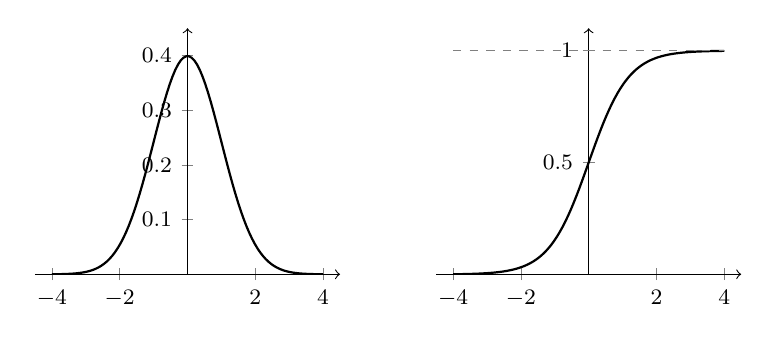
\begin{tikzpicture}[
      font=\footnotesize,
    ]
      \begin{axis}[
        name=pdf,
        width=0.45\linewidth,
        domain=-4:4,
        samples=100,
        axis lines=middle,
        inner axis line style={->},
        xmin=-4.5, xmax=4.5,
        ymax=0.45
      ]
        \addplot [thick, black] {exp(-0.5*x^2)/sqrt(2*pi)};
      \end{axis}
      
      \begin{axis}[
        at={(pdf.right of south east)},
        width=0.45\linewidth,
        xshift=0.1\linewidth,
        domain=-4:4,
        samples=100,
        axis lines=middle,
        inner axis line style={->},
        xmin=-4.5, xmax=4.5,
        ymax=1.1
      ]
        \addplot [thick, black] {1 / (1 + exp(-1.702 * x))};
        \draw[dashed, gray] (-4,1) -- (4,1);
      \end{axis}
    \end{tikzpicture}
  \caption{The p.d.f.\@ and d.f.\@ of the standard normal distribution.}
\end{figure}

The p.d.f.\@ of the normal distribution is obviously non-negative. We can show that the integral of the normal p.d.f.\@ is 1 by using the substitution \(z = \frac{x - \mu}{\sigma}\):
\[
  \int_{-\infty}^\infty \frac{1}{\sqrt{2\pi} \sigma} e^{-\frac{(x - \mu)^2}{2\sigma^2}}\,\mathrm{d}x = \frac{1}{\sqrt{2\pi}} \int_{-\infty}^\infty e^{-\frac{z^2}{2}}\,\mathrm{d}z \quad (z = \frac{x - \mu}{\sigma})
\]
By Theorem~\ref{thm:important_integrals}, we have
\[
  \int_{-\infty}^\infty e^{-\frac{z^2}{2}}\,\mathrm{d}z = 2 \int_{0}^{\infty} e^{-\frac{z^2}{2}}\,\mathrm{d}z = \sqrt{2\pi}.
\]
Therefore, the integral of the normal p.d.f.\@ is 1.

The d.f.\@ of \(X \sim \mathrm{N}(\mu, \sigma^2)\) is given by
\[
  F(x) = \frac{1}{\sqrt{2\pi} \sigma} \int_{-\infty}^x e^{-\frac{(t - \mu)^2}{2\sigma^2}}\,\mathrm{d}t, \quad -\infty < x < \infty,
\]
and the d.f.\@ of the standard normal distribution is given by
\[
  \Phi(z) = \frac{1}{\sqrt{2\pi}} \int_{-\infty}^z e^{-\frac{t^2}{2}}\,\mathrm{d}t, \quad -\infty < z < \infty.
\]

\begin{theorem}
  If \(X \sim \mathrm{N}(\mu, \sigma^2)\), then \(Z = \frac{X - \mu}{\sigma} \sim \mathrm{N}(0, 1)\).
\end{theorem}

\begin{proof}
  If \(X \sim \mathrm{N}(\mu, \sigma^2)\), and \(Z = \frac{X - \mu}{\sigma}\), then
  \begin{align*}
    P(Z \leq x) & = P\!\left(\frac{X - \mu}{\sigma} \leq x\right) \\
    & = P(X \leq \sigma x + \mu) \\
    & = \frac{1}{\sqrt{2\pi} \sigma} \int_{-\infty}^{\sigma x + \mu} e^{-\frac{(t - \mu)^2}{2\sigma^2}}\,\mathrm{d}t.
  \end{align*}
  Therefore,
  \[
    f_Z(x) = \frac{\mathrm{d}}{\mathrm{d}x} P(Z \leq x) = \frac{1}{\sqrt{2\pi}\sigma} e^{-\frac{(t - \mu)^2}{2\sigma^2}} \sigma \bigg|_{t = \sigma x + \mu} = \frac{1}{\sqrt{2\pi}} e^{-\frac{x^2}{2}}, \quad -\infty < x < \infty,
  \]
  which is the p.d.f.\@ of the standard normal distribution.
\end{proof}

\begin{example}
  Suppose that \(X \sim \mathrm{N}(10, 4)\). Find the value of \(P(10 < X < 13)\) and \(P(|X - 10| < 2)\).
\end{example}

\begin{solution}
  Since \(Z = \frac{X - 10}{2} \sim \mathrm{N}(0, 1)\), we have
  \[
    P(10 < X < 13) = P\!\left(0 < Z < \frac{3}{2}\right) = \Phi\!\left(\frac{3}{2}\right) - \Phi(0) = \Phi\!\left(\frac{3}{2}\right) - \frac{1}{2},
  \]
  and
  \[
    P(|X - 10| < 2) = P(8 < X < 12) = P\!\left(-1 < Z < 1\right) = \Phi(1) - \Phi(-1) = 2\Phi(1) - 1. \qedhere
  \]
\end{solution}

\begin{example}
  Suppose that \(X \sim \mathrm{N}(\mu, \sigma^2)\), \(P(X \leq -5) = 0.045\), and \(P(X \leq 3) = 0.618\). Find the values of \(\mu\) and \(\sigma\).
\end{example}

\begin{solution}
  Since \(P(X \leq -5) = 0.045\), we have
  \[
    P\!\left(\frac{X - \mu}{\sigma} \leq \frac{-5 - \mu}{\sigma}\right) = 0.045.
  \]
  Since \(P(X \leq 3) = 0.618\), we have
  \[
    P\!\left(\frac{X - \mu}{\sigma} \leq \frac{3 - \mu}{\sigma}\right) = 0.618.
  \]
  Let \(z_1 = \frac{-5 - \mu}{\sigma}\) and \(z_2 = \frac{3 - \mu}{\sigma}\). Then we have
  \[
    z_1 \approx -1.695, \quad z_2 \approx 0.300.
  \]
  Solving the equations, we have \(\mu = 1.80\) and \(\sigma \approx 4.01\).
\end{solution}

\section{Functions of Random Variables}

Mapping a discrete r.v.\@ to another discrete r.v.\@ will not change the nature of the distribution, i.e., the new r.v.\@ is still a discrete r.v.\@. However, mapping a continuous r.v.\@ to another r.v.\@ may not yield a continuous r.v.
\begin{example}
  Let \(X \sim \mathrm{N}(0, 1)\), \(Y = X^+\), i.e., \(Y = \max\{X, 0\}\). Then \(Y\) is not a continuous r.v.\@ since \(P(Y = 0) = P(X \leq 0) = \frac{1}{2} > 0\).
\end{example}
\begin{example}
  Suppose the p.d.f.\@ of a continuous r.v.\@ \(X\) is given by
  \[
    f_X(x) = \begin{cases}
      \frac{x}{8}, & 0 < x < 4, \\
      0, & \text{otherwise}.
    \end{cases}
  \]
  Find the p.d.f.\@ of \(Y = 2X + 1\).
\end{example}
\begin{solution}
  Since \(Y = 2X + 1\), we have
  \[
    F_Y(y) = P\{Y \leq y\} = P\{2X + 1 \leq y\} = P\left\{X \leq \frac{y - 1}{2}\right\} = \int_{-\infty}^{(y - 1)/2} f_X(x)\,\mathrm{d}x.
  \]
  \begin{enumerate}
    \item If \(y \leq 1\), we have \(F_Y(y) = 0\).
    \item If \(1 < y < 9\), we have
    \[
      F_Y(y) = \int_0^{(y - 1)/2} \frac{x}{8}\,\mathrm{d}x = \frac{(y - 1)^2}{64}.
    \]
    \item If \(y \geq 9\), we have \(F_Y(y) = 1\).
  \end{enumerate}
  Therefore,
  \[
    F_Y(y) = \begin{cases}
      0, & y \leq 1, \\
      \frac{(y - 1)^2}{64}, & 1 < y < 9, \\
      1, & y \geq 9.
    \end{cases}
  \]
  and
  \[
    f_Y(y) = F_Y'(y) = \begin{cases}
      0, & y \leq 1, \\
      \frac{y - 1}{32}, & 1 < y < 9, \\
      0, & y \geq 9.
    \end{cases} \qedhere
  \]
\end{solution}

\begin{theorem}
  Let \(X\) be a continuous r.v.\@ having p.d.f.\@ \(f_X\). Suppose that \(g(x)\) is a strictly monotonic, differentiable function of \(x\). Then the r.v.\@ \(Y = g(X)\) has p.d.f.\@
  \[
    f_Y(y) = \begin{cases}
      f_X(g^{-1}(y)) \left|\frac{\mathrm{d}}{\mathrm{d}y} g^{-1}(y)\right|, & \text{if } y = g(x) \text{ for some } x, \\
      0, & \text{otherwise},
    \end{cases}
  \]
  where \(g^{-1}(y)\) is defined to equal that the value of \(x\) such that \(g(x) = y\).
\end{theorem}

\begin{example}
  Assume that \(X \sim \mathrm{N}(0, 1)\), find the p.d.f.\@ of \(Y = X^2\).
\end{example}
\begin{solution}
  Since \(X \sim \mathrm{N}(0, 1)\), we have
  \[
    f_X(x) = \frac{1}{\sqrt{2\pi}} e^{-\frac{x^2}{2}}, \quad -\infty < x < \infty.
  \]
  \begin{enumerate}
    \item If \(y < 0\), we have \(f_Y(y) = 0\).
    \item If \(y \geq 0\), we have
    \begin{align*}
      f_Y(y) & = f_X(\sqrt{y}) \left|\frac{\mathrm{d}}{\mathrm{d}y} \sqrt{y}\right| + f_X(-\sqrt{y}) \left|\frac{\mathrm{d}}{\mathrm{d}y} (-\sqrt{y})\right| \\
      & = \frac{f_X(\sqrt{y}) + f_X(-\sqrt{y})}{2\sqrt{y}} \\
      & = \frac{1}{\sqrt{2 \pi}} y^{-\frac{1}{2}} e^{-\frac{y}{2}}.
    \end{align*}
  \end{enumerate}
  This indicates that \(Y\) has a \emph{chi-square distribution} with one degree of freedom, i.e., \(Y \sim \chi^2(1)\), which is a special case of the gamma distribution.
\end{solution}

\section{Expectation and Variance}

\begin{definition}[Expectation]\index{expectation}
  Suppose that the p.f.\@ of a discrete random variable \(X\) is \(P(X = x_k) = p_k, k = 1, 2, \dots\). The \emph{expectation} of \(X\) is defined as
  \[
    \mathbb{E}(X) = \sum_{k = 1}^\infty x_k p_k,
  \]
  if \(\sum_{k = 1}^\infty x_k p_k\) is absolutely convergent.
\end{definition}

\begin{definition}[Expectation]\index{expectation}
  Suppose that the p.d.f.\@ of \(X\) is \(f(x)\). The \emph{expectation} of \(X\) is defined as
  \[
    \mathbb{E}(X) = \int_{-\infty}^\infty x f(x)\,\mathrm{d}x,
  \]
  if the integral converges.
\end{definition}

The expectation of the uniform distribution \(X \sim \mathrm{U}(a, b)\) is given by
\[
  \mathbb{E}(X) = \int_a^b x \frac{1}{b - a}\,\mathrm{d}x = \frac{a + b}{2}.
\]

The expectation of the exponential distribution \(X \sim \mathrm{Exp}(\lambda)\) is given by
\begin{align*}
  \mathbb{E}(X) & = \int_0^\infty x \lambda e^{-\lambda x}\,\mathrm{d}x = \int_0^\infty x\,\mathrm{d}(-e^{-\lambda x}) \\
  & = \left[-x e^{-\lambda x}\right]_0^\infty + \int_0^\infty e^{-\lambda x}\,\mathrm{d}x = \frac{1}{\lambda},
\end{align*}
which can be interpreted as the average frequency of the occurrence of the event.

The expectation of the normal distribution \(X \sim \mathrm{N}(\mu, \sigma^2)\) can be calculated by
\[
  \mathbb{E}(X) = \int_{-\infty}^\infty x \frac{1}{\sqrt{2\pi} \sigma} e^{-\frac{(x - \mu)^2}{2\sigma^2}}\,\mathrm{d}x.
\]
Let \(y = \frac{x - \mu}{\sigma}\), then
\begin{align*}
  \mathbb{E}(X) & = \int_{-\infty}^\infty (\sigma y + \mu) \frac{1}{\sqrt{2\pi}} e^{-\frac{y^2}{2}}\,\mathrm{d}y \\
  & = \sigma \int_{-\infty}^\infty y \frac{1}{\sqrt{2\pi}} e^{-\frac{y^2}{2}}\,\mathrm{d}y + \mu \int_{-\infty}^\infty \frac{1}{\sqrt{2\pi}} e^{-\frac{y^2}{2}}\,\mathrm{d}y \\
  & = 0 + \mu = \mu.
\end{align*}

\begin{theorem}
  The mathematical expectation of a function \(g(X)\) of a r.v.\@ \(X\) can be calculated by
  \[
    \mathbb{E}[g(X)] = \begin{cases}
      \sum_{i = 1}^\infty g(x_i) p(x_i), & \text{if } X \text{ is discrete}, \\
      \int_{-\infty}^\infty g(x) f(x)\,\mathrm{d}x, & \text{if } X \text{ is continuous}.
    \end{cases}
  \]
  The expectation \(\mathbb{E}[g(X)]\) will exist if and only if \(\sum_{i = 1}^\infty |g(x_i)| p(x_i) < \infty\) for discrete \(X\) or \(\int_{-\infty}^\infty |g(x)| f(x)\,\mathrm{d}x < \infty\) for continuous \(X\).
\end{theorem}

\begin{proposition}
  Some properties of expectation are as follows:
  \begin{enumerate}
    \item \(\mathbb{E}(c) = c\) for any constant \(c\).
    \item \(\mathbb{E}(cX) = c \mathbb{E}(X)\) for any constant \(c\).
    \item \(\mathbb{E}(X + Y) = \mathbb{E}(X) + \mathbb{E}(Y)\) for any r.v.\@ \(X\) and \(Y\).
    \item \(\mathbb{E}[X - \mathbb{E}(X)]^2 = \mathbb{E}[X^2 - 2X\mathbb{E}(X) + (\mathbb{E}(X))^2] = \mathbb{E}(X^2) - [\mathbb{E}(X)]^2\).
  \end{enumerate}
\end{proposition}

\begin{example}
  Suppose that \(X \sim \mathrm{N}(\mu, \sigma^2)\), find the expectation of \(Y = e^X\).
\end{example}
\begin{solution}
  Since \(X \sim \mathrm{N}(\mu, \sigma^2)\), we have
  \begin{align*}
    \mathbb{E}(Y) & = \mathbb{E}(e^X) = \int_{-\infty}^\infty e^x \frac{1}{\sqrt{2\pi} \sigma} e^{-\frac{(x - \mu)^2}{2\sigma^2}}\,\mathrm{d}x \\
    & = \int_{-\infty}^\infty \frac{1}{\sqrt{2\pi} \sigma} \exp\left(-\frac{x^2 -2(\mu + \sigma^2)x + (\mu + \sigma^2)^2 - 2\mu\sigma^2 - \sigma^4}{2\sigma^2}\right)\,\mathrm{d}x \\
    & = e^{\mu + \frac{\sigma^2}{2}} \int_{-\infty}^\infty \frac{1}{\sqrt{2\pi} \sigma} e^{-\frac{(x - \mu - \sigma^2)^2}{2\sigma^2}}\,\mathrm{d}x = e^{\mu + \frac{\sigma^2}{2}}. \qedhere
  \end{align*}
\end{solution}

\begin{definition}[Variance]\index{variance}
  The \emph{variance} of a r.v.\@ \(X\) is defined as
  \[
    \mathrm{Var}(X) = \mathbb{E}[X - \mathbb{E}(X)]^2 = \mathbb{E}(X^2) - [\mathbb{E}(X)]^2,
  \]
  if the expectation exists.
\end{definition}

\begin{proposition}
  Some properties of variance are as follows:
  \begin{enumerate}
    \item \(\mathrm{Var}(c) = 0\) for any constant \(c\).
    \item \(\mathrm{Var}(cX) = c^2 \mathrm{Var}(X)\) for any constant \(c\).
    \item \(\mathrm{Var}(X) = 0\) if and only if \(P(X = \mathbb{E}(X)) = 1\).
  \end{enumerate}
\end{proposition}

\begin{theorem}[Chebyshev's Inequality]\index{Chebyshev's inequality}
  Suppose that \(\mathbb{E}(X) = \mu\) and \(\mathrm{Var}(X) = \sigma^2\). Then for any \(\varepsilon > 0\), we have
  \[
    P(|X - \mu| \geq \varepsilon) \leq \frac{\sigma^2}{\varepsilon^2}.
  \]
\end{theorem}

\begin{example}[Standarization]
  Suppose that the expectation and variance of a r.v.\@ \(X\) are \(\mathbb{E}(X)\) and \(\mathrm{Var}(X)\). Find the expectation and variance of \(Y = \frac{X - \mathbb{E}(X)}{\sqrt{\mathrm{Var}(X)}}\).
\end{example}
\begin{solution}
  Since \(Y = \frac{X - \mathbb{E}(X)}{\sqrt{\mathrm{Var}(X)}}\), we have
  \[
    \mathbb{E}(Y) = \frac{\mathbb{E}(X) - \mathbb{E}(X)}{\sqrt{\mathrm{Var}(X)}} = 0,
  \]
  and
  \[
    \mathrm{Var}(Y) = \frac{\mathrm{Var}[X - \mathbb{E}(X)]}{\mathrm{Var}(X)} = \frac{\mathrm{Var}(X)}{\mathrm{Var}(X)} = 1. \qedhere
  \]
\end{solution}

\begin{table}[tbp]
  \centering
  \caption{Summary of Common Discrete Distributions}
  \label{tab:common_distributions}
  \scriptsize
  \begin{tabular}{l l l l l}
    \toprule
    Distribution & Parameter(s) & Probability Mass Function & Expectation & Variance \\
    \midrule
    Bernoulli & $p$ & $P(X = 1) = p, P(X = 0) = 1 - p$ & $p$ & $p(1 - p)$ \\
    Binomial & $n, p$ & $\binom{n}{k} p^k (1 - p)^{n - k}$ & $np$ & $np(1 - p)$ \\
    Poisson & $\lambda$ & $\frac{\lambda^k e^{-\lambda}}{k!}$ & $\lambda$ & $\lambda$ \\
    Geometric & $p$ & $p (1 - p)^{k - 1}$ & $\frac{1}{p}$ & $\frac{1 - p}{p^2}$ \\
    Pascal & $k, p$ & $\binom{n - 1}{k - 1} p^k (1 - p)^{n - k}$ & $\frac{k}{p}$ & $\frac{k(1 - p)}{p^2}$ \\
    Hypergeometric & $N, M, n$ & $\frac{\binom{M}{m} \binom{N - M}{n - m}}{\binom{N}{n}}$ & $\frac{nM}{N}$ & $\frac{nM(N - M)(N - n)}{N^2(N - 1)}$ \\
    \bottomrule
  \end{tabular}
\end{table}

\begin{table}[tbp]
  \centering
  \caption{Summary of Common Continuous Distributions}
  \scriptsize
  \begin{tabular}{l l l l l l}
    \toprule
    Distribution & Parameter(s) & p.d.f.\@ & d.f.\@ & Expectation & Variance \\
    \midrule
    Uniform & \(a < b\) & \(\frac{1}{b - a}\) for \(a < x < b\) & \(\frac{x - a}{b - a}\) for \(a < x < b\) & \(\frac{a + b}{2}\) & \(\frac{(b - a)^2}{12}\) \\
    Exponential & \(\lambda > 0\) & \(\lambda e^{-\lambda x}\) for \(x > 0\) & \(1 - e^{-\lambda x}\) for \(x > 0\) & \(\frac{1}{\lambda}\) & \(\frac{1}{\lambda^2}\) \\
    Normal & \(\mu, \sigma\) & \(\frac{1}{\sqrt{2\pi} \sigma} e^{-\frac{(x - \mu)^2}{2\sigma^2}}\) & \(\int_{-\infty}^x f(t)\,dt\) & \(\mu\) & \(\sigma^2\) \\
    \bottomrule
  \end{tabular}
\end{table}

\chapter{Random Vector}

\section{Bivariate Random Variables}

\begin{definition}[Bivariate Random Variable]\index{bivariate random variable}
  A pair of random variables \((X, Y)\) defined on the same sample space \(\Omega\) is called a \emph{bivariate random variable}.
\end{definition}

\begin{definition}[Joint Distribution Function]\index{joint distribution function}
  The \emph{joint distribution function} (joint d.f.\@) of a bivariate random variable \((X, Y)\) is defined as
  \[
    F(x, y) = P\!\left(\{X \leq x\} \cap \{Y \leq y\}\right) = P(X \leq x, Y \leq y).
  \]
\end{definition}

\begin{proposition}
  Some properties of the joint d.f.\@ \(F(x, y)\) of a bivariate random variable \((X, Y)\) are as follows:
  \begin{enumerate}
    \item (Monotonicity) If \(y_2 > y_1\), then \(F(x, y_2) \geq F(x, y_1)\) for any \(x\); if \(x_2 > x_1\), then \(F(x_2, y) \geq F(x_1, y)\) for any \(y\).
    \item (Right-continuity) \(\lim_{x \to x_0^+} F(x, y) = F(x_0, y)\) for any \(y\); \(\lim_{y \to y_0^+} F(x, y) = F(x, y_0)\) for any \(x\).
    \item \(0 \leq F(x, y) \leq 1\) for all \(x, y \in \mathbb{R}\), and
    \begin{align*}
      F(x, -\infty) = \lim_{y \to -\infty} F(x, y) = 0, &\quad F(-\infty, y) = \lim_{x \to -\infty} F(x, y) = 0, \\
      F(-\infty, -\infty) = \lim_{x \to -\infty} \lim_{y \to -\infty} F(x, y) = 0, &\quad F(\infty, \infty) = \lim_{x \to \infty} \lim_{y \to \infty} F(x, y) = 1.
    \end{align*}
    \item (Non-negativity) For any \(x_1 < x_2\) and \(y_1 < y_2\), we have
    \begin{align*}
      &P(x_1 < X \leq x_2, y_1 < Y \leq y_2) \\
      &= F(x_2, y_2) - F(x_2, y_1) - F(x_1, y_2) + F(x_1, y_1) \geq 0.
    \end{align*}
  \end{enumerate}
\end{proposition}

\begin{example}
  The joint d.f.\@ of a bivariate random variable \((X, Y)\) is given by
  \[
    F(x, y) = A \left(B + \arctan\frac{x}{2}\right) \left(C + \arctan\frac{y}{2}\right), \quad x, y \in \mathbb{R}.
  \]
  \begin{enumerate}
    \item Find the values of the constants \(A, B, C\).
    \item Determine the value of \(P(0 < X \leq 2, 0 < Y \leq 3)\).
  \end{enumerate}
\end{example}
\begin{solution}
  \begin{enumerate}
    \item Since \(F(x, y)\) is a joint d.f.\@, it must satisfy the properties stated in the previous proposition. In particular, we have
    \[
      \begin{cases}
        F(-\infty, y) = 0 \implies A (B - \frac{\pi}{2}) (C + \arctan\frac{y}{2}) = 0, \\
        F(x, -\infty) = 0 \implies A (B + \arctan\frac{x}{2}) (C - \frac{\pi}{2}) = 0, \\
        F(\infty, \infty) = 1 \implies A (B + \frac{\pi}{2}) (C + \frac{\pi}{2}) = 1.
      \end{cases}
    \]
    Solving these equations, we find \(A = \frac{1}{\pi^2}\), \(B = \frac{\pi}{2}\), and \(C = \frac{\pi}{2}\).
    \item We have
    \[
      P(0 < X \leq 2, 0 < Y \leq 3) = F(2, 3) - F(2, 0) - F(0, 3) + F(0, 0)
    \]
    Substituting the values of \(A, B, C\) and evaluating the joint d.f.\@ at the specified points, we can compute the desired probability. \qedhere
  \end{enumerate}
\end{solution}

\begin{definition}[Joint Probability Function]\index{joint probability function}
  For discrete bivariate random vectors \((X, Y)\), whose possible values are a countable set of points \((x_i, y_j) (i, j = 1, 2, \dots)\), the \emph{joint probability function} (joint p.f.\@) is defined as
  \[
    p(x, y) = P(X = x, Y = y).
  \]
\end{definition}

\begin{proposition}
  For a discrete bivariate random variable \((X, Y)\) with joint p.f.\@ \(p_{ij} = P(X = x_i, Y = y_j)\), we have
  \begin{enumerate}
    \item \(p_{ij} \geq 0\) for all \(i, j\).
    \item \(\sum_{i=1}^\infty \sum_{j=1}^\infty p_{ij} = 1\).
    \item The joint d.f.\@ \(F(x, y)\) can be expressed in terms of the joint p.f.\@ as
    \[
      F(x, y) = P(X \leq x, Y \leq y) = \sum_{x_i \leq x} \sum_{y_j \leq y} p_{ij}.
    \]
  \end{enumerate}
\end{proposition}

\begin{example}
  Assume that \(Y \sim \mathrm{N}(0, 1)\). Find the joint p.f.\@ of
  \[
    X_1 = \begin{cases}
      0, & |Y| \geq 1, \\
      1, & |Y| < 1,
    \end{cases}
    X_2 = \begin{cases}
      0, & |Y| \geq 2, \\
      1, & |Y| < 2.
    \end{cases}
  \]
\end{example}
\begin{solution}
  \begin{align*}
    P(X_1 = 0, X_2 = 0) &= P(|Y| \geq 2) = 2P(Y \geq 2) = 2(1 - \Phi(2)), \\
    P(X_1 = 0, X_2 = 1) &= P(|Y| \geq 1, |Y| < 2) = P(1 \leq |Y| < 2) = 2(\Phi(2) - \Phi(1)), \\
    P(X_1 = 1, X_2 = 0) &= P(|Y| < 1, |Y| \geq 2) = 0, \\
    P(X_1 = 1, X_2 = 1) &= P(|Y| < 1) = 2\Phi(1) - 1. \qedhere
  \end{align*}
\end{solution}

\begin{definition}[Joint Probability Density Function]\index{joint probability density function}\index{jointly continuous}
  For a bivariate random variable \((X, Y)\), if there exists a non-negative function \(f(x, y)\) such that
  \[
    F(x, y) = P(X \leq x, Y \leq y) = \int_{-\infty}^x \int_{-\infty}^y f(u, v) \, \mathrm{d}u \, \mathrm{d}v,
  \]
  for all \(x, y \in \mathbb{R}\), then \(X\) and \(Y\) are called \emph{jointly continuous}, and the function \(f(x, y)\) is called the \emph{joint probability density function} (joint p.d.f.\@) of \((X, Y)\).
\end{definition}

\begin{proposition}
  For a jointly continuous bivariate random variable \((X, Y)\) with joint p.d.f.\@ \(f(x, y)\), we have
  \begin{enumerate}
    \item \(f(x, y) \geq 0\) for all \(x, y \in \mathbb{R}\).
    \item \(\iint_{\mathbb{R}^2} f(x, y) \, \mathrm{d}x \, \mathrm{d}y = 1\).
    \item If \(f(x, y)\) is continuous at a point \((x, y)\), then
    \[
      f(x, y) = \frac{\partial^2 F(x, y)}{\partial x \partial y} = \lim_{\Delta x,\Delta y\to0^+}\frac{P(x<X\le x+\Delta x,\ y<Y\le y+\Delta y)}{\Delta x,\Delta y}.
    \]
    \item For any \(G \subseteq \mathbb{R}^2\), we have
    \[
      P\{(X, Y) \in G\} = \iint_G f(x, y) \, \mathrm{d}x \, \mathrm{d}y.
    \]
  \end{enumerate}
\end{proposition}

\begin{definition}[Bivariate Uniform Distribution]\index{bivariate uniform distribution}
  A bivariate random variable \((X, Y)\) is said to have a \emph{bivariate uniform distribution} on a measurable region \(R\) with finite positive area if its joint p.d.f.\@ is given by
  \[
    f(x, y) = \begin{cases}
      \frac{1}{\text{area}(R)}, & (x, y) \in R, \\
      0, & (x, y) \notin R.
    \end{cases}
  \]
\end{definition}

\begin{definition}[Bivariate Normal Distribution]\index{bivariate normal distribution}
  A bivariate random variable \((X, Y)\) is said to have a \emph{bivariate normal distribution} with parameters \(\mu_1, \mu_2, \sigma_1 > 0, \sigma_2 > 0\), and \(|\rho| < 1\) if its joint p.d.f.\@ is given by
  \[
    f(x, y) = \frac{1}{2\pi \sigma_1 \sigma_2 \sqrt{1 - \rho^2}} e^{-\frac{1}{2(1 - \rho^2)} \left[\frac{(x - \mu_1)^2}{\sigma_1^2} - 2\rho \frac{(x - \mu_1)(y - \mu_2)}{\sigma_1 \sigma_2} + \frac{(y - \mu_2)^2}{\sigma_2^2}\right]}.
  \]
  We denote this distribution by \((X, Y) \sim \mathrm{N}(\mu_1, \mu_2; \sigma_1^2, \sigma_2^2; \rho)\).
\end{definition}

\begin{example}
  Suppose that \((X, Y) \sim f(x, y)\) with
  \[
    f(x, y) = \begin{cases}
      A e^{-(2x + 3y)}, & x \geq 0, y \geq 0 \\
      0, & \text{otherwise}.
    \end{cases}
  \]
  \begin{enumerate}
    \item Find the value of the constant \(A\).
    \item Calculate the probability \(P(X < 2, Y < 1)\).
  \end{enumerate}
\end{example}
\begin{solution}
  \begin{enumerate}
    \item Since \(f(x, y)\) is a joint p.d.f.\@, it must satisfy the property that \(\iint_{\mathbb{R}^2} f(x, y) \, \mathrm{d}x \, \mathrm{d}y = 1\). Therefore, we have
    \begin{align*}    
      \iint_{\mathbb{R}^2} f(x, y) \, \mathrm{d}x \, \mathrm{d}y &= \int_0^\infty \int_0^\infty A e^{-(2x + 3y)} \, \mathrm{d}x \, \mathrm{d}y \\
      &= A \int_0^\infty e^{-2x} \, \mathrm{d}x \int_0^\infty e^{-3y} \, \mathrm{d}y \\
      &= A \left(-\frac{1}{2} e^{-2x}\right)\Big|_0^\infty \left(-\frac{1}{3} e^{-3y}\right)\Big|_0^\infty = \frac{1}{6} A = 1.
    \end{align*}
    Solving for \(A\), we find \(A = 6\).
    \item We can compute the desired probability as follows:
    \begin{align*}
      P(X < 2, Y < 1) &= \iint_{0 \leq x < 2, 0 \leq y < 1} f(x, y) \, \mathrm{d}x \, \mathrm{d}y \\
      &= \int_0^2 \int_0^1 6 e^{-(2x + 3y)} \, \mathrm{d}y \, \mathrm{d}x = 6 \int_0^2 e^{-2x} \, \mathrm{d}x \int_0^1 e^{-3y} \, \mathrm{d}y \\
      &= 6 \left(-\frac{1}{2} e^{-2x}\right)\Big|_0^2 \left(-\frac{1}{3} e^{-3y}\right)\Big|_0^1 = (1 - e^{-3})(1 - e^{-4}). \qedhere
    \end{align*}
  \end{enumerate}
\end{solution}

\begin{example}
  Suppose that the joint p.d.f.\@ of \(X, Y\) is given by
  \[
    f(x, y) = \begin{cases}
      e^{-y}, & 0 < x < y \\
      0, & \text{otherwise}.
    \end{cases}
  \]
  Calculate the probability \(P(X + Y \leq 1)\).
\end{example}
\begin{solution}
  \begin{align*}
    P(X + Y \leq 1) &= \iint_{x + y \leq 1} f(x, y) \, \mathrm{d}x \, \mathrm{d}y \\
    &= \int_0^\frac{1}{2} \mathrm{d}x \int_x^{1 - x} e^{-y} \, \mathrm{d}y \\
    &= 1 + e^{-1} - 2e^{-\frac{1}{2}}. \qedhere
  \end{align*}
\end{solution}

\section{Marginal Distribution}

\begin{definition}[Marginal Distribution]\index{marginal distribution}
  Suppose that \(F(x, y)\) is the joint d.f.\@ of a bivariate random variable \((X, Y)\). The \emph{marginal distributions} of \(X\) and \(Y\) are defined as
  \[
    F_X(x) = P(X \leq x) = F(x, \infty), \quad F_Y(y) = P(Y \leq y) = F(\infty, y).
  \]
\end{definition}

In the case of discrete bivariate random variables with joint p.f.\@ \(p_{ij} = P(X = x_i, Y = y_j)\), the marginal distributions can be expressed in terms of the joint p.f.\@ as
\[
  F_X(x) = P(X \leq x) = \sum_{x_i \leq x} \sum_{j=1}^\infty p_{ij}, \quad F_Y(y) = P(Y \leq y) = \sum_{i=1}^\infty \sum_{y_j \leq y} p_{ij}.
\]
The marginal p.f.\@ of \(X\) and \(Y\) are given by
\[
  p_{i \cdot} = P(X = x_i) = \sum_{j=1}^\infty p_{ij}, \quad p_{\cdot j} = P(Y = y_j) = \sum_{i=1}^\infty p_{ij}.
\]

In the case of jointly continuous bivariate random variables, the marginal distributions can be expressed in terms of the joint p.d.f.\@ as
\begin{align*}
  F_X(x) &= P(X \leq x) = \int_{-\infty}^x \left[\int_{-\infty}^\infty f(u, y) \, \mathrm{d}y \right] \mathrm{d}u, \\
  F_Y(y) &= P(Y \leq y) = \int_{-\infty}^y \left[\int_{-\infty}^\infty f(x, v) \, \mathrm{d}x \right] \mathrm{d}v.
\end{align*}
The marginal p.d.f.\@ of \(X\) and \(Y\) is given by
\[
  f_X(x) = \int_{-\infty}^\infty f(x, y) \, \mathrm{d}y, \quad f_Y(y) = \int_{-\infty}^\infty f(x, y) \, \mathrm{d}x.
\]

\begin{example}
  Suppose that \(X, Y\) have the uniform distribution on the region \(D_1 = \{(x, y), x^2 + y^2 \leq 1\}\). Find the marginal p.d.f.\@ of \(X\).
\end{example}
\begin{solution}
  Since \(X, Y\) have the uniform distribution on the region \(D_1\), we have
  \[
    f(x, y) = \begin{cases}
      \frac{1}{\pi}, & x^2 + y^2 \leq 1, \\
      0, & \text{otherwise}.
    \end{cases}
  \]
  \begin{enumerate}
    \item When \(|x| > 1\), \(f(x, y) = 0\) for all \(y\), so \(f_X(x) = 0\).
    \item When \(|x| \leq 1\), we have
    \[
      f_X(x) = \int_{-\sqrt{1 - x^2}}^{\sqrt{1 - x^2}} \frac{1}{\pi} \, \mathrm{d}y = \frac{2}{\pi}\sqrt{1 - x^2}.
    \]
  \end{enumerate}
  That is,
  \[
    f_X(x) = \begin{cases}
      \frac{2}{\pi}\sqrt{1 - x^2}, & -1 \leq x \leq 1, \\
      0, & \text{otherwise}.
    \end{cases} \qedhere
  \]
\end{solution}

\begin{proposition}
  If \((X, Y) \sim \mathrm{U}([a, b] \times [c, d])\), then \(X \sim \mathrm{U}(a, b)\) and \(Y \sim \mathrm{U}(c, d)\).
\end{proposition}

\begin{proposition}
  If \((X, Y) \sim \mathrm{N}(\mu_1, \mu_2; \sigma_1^2, \sigma_2^2; \rho)\), then \(X \sim \mathrm{N}(\mu_1, \sigma_1^2)\) and \(Y \sim \mathrm{N}(\mu_2, \sigma_2^2)\).
\end{proposition}
\begin{proof}
  Since \((X, Y) \sim \mathrm{N}(\mu_1, \mu_2; \sigma_1^2, \sigma_2^2; \rho)\), the joint p.d.f.\@ of \(X\) and \(Y\) is given by
  \[
    f(x, y) = \frac{1}{2\pi \sigma_1 \sigma_2 \sqrt{1 - \rho^2}} e^{-\frac{1}{2(1 - \rho^2)} \left[\frac{(x - \mu_1)^2}{\sigma_1^2} - 2\rho \frac{(x - \mu_1)(y - \mu_2)}{\sigma_1 \sigma_2} + \frac{(y - \mu_2)^2}{\sigma_2^2}\right]}.
  \]
  Since
  \[
    \frac{(y - \mu_2)^2}{\sigma_2^2} - 2\rho \frac{(x - \mu_1)(y - \mu_2)}{\sigma_1 \sigma_2} = \left(\frac{y - \mu_2}{\sigma_2} - \rho \frac{x - \mu_1}{\sigma_1}\right)^2 - \rho^2 \frac{(x - \mu_1)^2}{\sigma_1^2},
  \]
  we can calculate the marginal p.d.f.\@ of \(X\) as follows:
  \begin{align*}
    f_X(x) &= \int_{-\infty}^\infty f(x, y) \, \mathrm{d}y \\
    &= \int_{-\infty}^\infty \frac{1}{2\pi \sigma_1 \sigma_2 \sqrt{1 - \rho^2}} e^{-\frac{1}{2(1 - \rho^2)} \left[\frac{(x - \mu_1)^2}{\sigma_1^2} + \left(\frac{y - \mu_2}{\sigma_2} - \rho \frac{x - \mu_1}{\sigma_1}\right)^2 - \rho^2 \frac{(x - \mu_1)^2}{\sigma_1^2}\right]} \, \mathrm{d}y \\
    &= \frac{1}{2\pi \sigma_1 \sigma_2 \sqrt{1 - \rho^2}} e^{-\frac{(x - \mu_1)^2}{2\sigma_1^2}} \int_{-\infty}^\infty e^{-\frac{1}{2(1 - \rho^2)}\left(\frac{y - \mu_2}{\sigma_2} - \rho \frac{x - \mu_1}{\sigma_1}\right)^2} \, \mathrm{d}y.
  \end{align*}
  Let \(t = \frac{1}{\sqrt{1 - \rho^2}} \left(\frac{y - \mu_2}{\sigma_2} - \rho \frac{x - \mu_1}{\sigma_1}\right)\), then \(\mathrm{d}t = \frac{1}{\sqrt{1 - \rho^2}} \frac{1}{\sigma_2} \, \mathrm{d}y\). Therefore,
  \[
    f_X(x) = \frac{1}{2\pi \sigma_1} e^{-\frac{(x - \mu_1)^2}{2\sigma_1^2}} \int_{-\infty}^\infty e^{-\frac{t^2}{2}} \, \mathrm{d}t = \frac{1}{\sqrt{2\pi} \sigma_1} e^{-\frac{(x - \mu_1)^2}{2\sigma_1^2}}.
  \]
  So \(X \sim \mathrm{N}(\mu_1, \sigma_1^2)\). By symmetry, we can also show that \(Y \sim \mathrm{N}(\mu_2, \sigma_2^2)\).
\end{proof}

\section{Conditional Distribution}

\begin{definition}[Conditional Probability Function]\index{conditional probability function}
  For a discrete bivariate random variable \((X, Y)\) with joint p.f.\@ \(p_{ij} = P(X = x_i, Y = y_j)\), the \emph{conditional probability function} (conditional p.f.\@) of \(X\) given \(Y = y_j\) is defined as
  \[
    p_{i|j} = P(X = x_i | Y = y_j) = \frac{P(X = x_i, Y = y_j)}{P(Y = y_j)} = \frac{p_{ij}}{p_{\cdot j}},
  \]
  provided that \(p_{\cdot j} > 0\).
\end{definition}

\begin{definition}[Conditional Distribution Function]\index{conditional distribution function}
  For a discrete bivariate random variable \((X, Y)\) with joint p.f.\@ \(p_{ij} = P(X = x_i, Y = y_j)\), the \emph{conditional distribution function} (conditional d.f.\@) of \(X\) given \(Y = y_j\) is defined as
  \[
    F_{X | Y}(x | y_j) = P\{X \leq x | Y = y_j\} = \frac{\sum_{x_i \leq x} p_{ij}}{p_{\cdot j}}
  \]
  provided that \(p_{\cdot j} > 0\).
\end{definition}

\begin{definition}[Conditional Probability Density Function]\index{conditional probability density function}
  For a jointly continuous bivariate random variable \((X, Y)\) with joint p.d.f.\@ \(f(x, y)\), the \emph{conditional probability density function} (conditional p.d.f.\@) of \(X\) given \(Y = y\) is defined as
  \[
    f_{X|Y}(x | y) = \frac{f(x, y)}{f_Y(y)},
  \]
  where \(f_Y(y)\) is the marginal p.d.f.\@ of \(Y\), provided that \(f_Y(y) > 0\).
\end{definition}

For a continuous random variable $Y$, the probability of exactly observing $Y = y$ is zero ($P(Y=y) = 0$). To define the conditional distribution of $X$ given $Y=y$, we must therefore consider an interval around $y$ and take the limit as the interval length goes to zero to capture the behavior of $X$ as $Y$ approaches $y$.

\begin{definition}[Conditional Distribution Function]\index{conditional distribution function}
  In the case of a jointly continuous bivariate random variable \((X, Y)\) with joint p.d.f.\@ \(f(x, y)\), for any \(x\), the limit
  \[
    F_{X | Y}(x | y) = \lim_{\varepsilon \to 0^+} P\{X \leq x | y - \varepsilon < Y \leq y + \varepsilon\} = \int_{-\infty}^{x} \frac{f(u, y)}{f_Y(y)} \, \mathrm{d}u
  \]
  is called \emph{conditional distribution function} (conditional d.f.\@) of \(X\) given \(Y = y\) if it exists, provided that \(f_Y(y) > 0\).
\end{definition}

\begin{example}
  Suppose that the number \(X\) is taken randomly from the interval \((0, 1)\). When \(X = x (0 < x < 1)\) is given, the number \(Y\) is taken randomly from the interval \((x, 1)\). Find the marginal p.d.f.\@ \(f_Y(y)\) of \(Y\).
\end{example}
\begin{solution}
  Since \(X\) is taken randomly from the interval \((0, 1)\), the p.d.f.\@ of \(X\) is given by
  \[
    f_X(x) = \begin{cases}
      1, & 0 < x < 1, \\
      0, & \text{otherwise}.
    \end{cases}
  \]
  For any \(0 < x < 1\), when \(X = x\) is given, the p.d.f.\@ of \(Y\) is given by
  \[
    f_{Y|X}(y | x) = \begin{cases}
      \frac{1}{1 - x}, & x < y < 1, \\
      0, & \text{otherwise}.
    \end{cases}
  \]
  Therefore, the joint p.d.f.\@ of \(X\) and \(Y\) is given by
  \[
    f(x, y) = f_X(x) f_{Y|X}(y | x) = \begin{cases}
      \frac{1}{1 - x}, & 0 < x < y < 1, \\
      0, & \text{otherwise}.
    \end{cases}
  \]
  Thus, the marginal p.d.f.\@ of \(Y\) is given by
  \[
    f_Y(y) = \int_{-\infty}^\infty f(x, y) \, \mathrm{d}x = \begin{cases}
      \int_0^y \frac{1}{1 - x} \, \mathrm{d}x = -\ln(1 - y), & 0 < y < 1, \\
      0, & \text{otherwise}.
    \end{cases} \qedhere
  \]
\end{solution}

\begin{example}
  Suppose that the joint p.d.f.\@ of \(X, Y\) is given by
  \[
    f(x, y) = \begin{cases}
      3x, & 0 < x < 1, 0 < y < x, \\
      0, & \text{otherwise}.
    \end{cases}
  \]
  \begin{enumerate}
    \item Find the marginal p.d.f.\@ of \(X\) and \(Y\).
    \item Find the conditional p.d.f.\@ of \(X\) and \(Y\).
  \end{enumerate}
\end{example}
\begin{solution}
  \begin{enumerate}
    \item The marginal p.d.f.\@ of \(X\) is given by
    \[
      f_X(x) = \int_{-\infty}^\infty f(x, y) \, \mathrm{d}y = \int_0^x 3x \, \mathrm{d}y = 3x^2, \quad 0 < x < 1,
    \]
    and the marginal p.d.f.\@ of \(Y\) is given by
    \[
      f_Y(y) = \int_{-\infty}^\infty f(x, y) \, \mathrm{d}x = \int_y^1 3x \, \mathrm{d}x = \frac{3}{2}(1 - y^2), \quad 0 < y < 1.
    \]
    For other values of \(x\) and \(y\), the marginal p.d.f.\@s are zero.
    \item If \(0 < y < 1\), the conditional p.d.f.\@ of \(X\) given \(Y = y\) is given by
    \[
      f_{X|Y}(x | y) = \frac{f(x, y)}{f_Y(y)} = \begin{cases}
        \frac{2x}{1 - y^2}, & y < x < 1, \\
        0, & \text{otherwise}.
      \end{cases}
    \]
    If \(0 < x < 1\), the conditional p.d.f.\@ of \(Y\) given \(X = x\) is given by
    \[
      f_{Y|X}(y | x) = \frac{f(x, y)}{f_X(x)} = \begin{cases}
        \frac{1}{x}, & 0 < y < x, \\
        0, & \text{otherwise}.
      \end{cases} \qedhere
    \]
  \end{enumerate}
\end{solution}

\begin{proposition}
  Suppose that \((X, Y) \sim \mathrm{N}(\mu_1, \mu_2; \sigma_1^2, \sigma_2^2; \rho)\). Then the conditional distribution of \(X\) given \(Y = y\) is a normal distribution with mean \(\mu_1 + \rho \frac{\sigma_1}{\sigma_2} (y - \mu_2)\) and variance \((1 - \rho^2) \sigma_1^2\).
\end{proposition}

\section{Independence of Variables}

\begin{definition}[Independence]\index{independence}
  A bivariate random variable \((X, Y)\) is said to be \emph{independent} if for any \(x, y \in \mathbb{R}\), we have
  \[
    P(X \leq x, Y \leq y) = P(X \leq x) P(Y \leq y),
  \]
  or equivalently,
  \[
    F(x, y) = F_X(x) F_Y(y).
  \]
\end{definition}

\begin{proposition}
  A discrete bivariate random variable \((X, Y)\) with joint p.f.\@ \(p_{ij} = P(X = x_i, Y = y_j)\) is independent if and only if there exist two sequences of non-negative numbers \(\{p_{i \cdot}\}\) and \(\{p_{\cdot j}\}\) such that \(p_{ij} = p_{i \cdot} p_{\cdot j}\) for all \(i, j\).
\end{proposition}
\begin{proof}
  \((\Rightarrow)\) Suppose that \((X, Y)\) is independent. Then for any \(x_1 < x_2\) and \(y_1 < y_2\), we have
  \[
    P\{x_1 < X \leq x_2, y_1 < Y \leq y_2\} = P\{x_1 < X \leq x_2\} P\{y_1 < Y \leq y_2\}.
  \]
  For any \(i, j\), we have
  \begin{align*}
    p_{ij} &= P\{X = x_i, Y = y_j\} \\
    &= \lim_{n, m \to \infty} P\{x_i - \frac{1}{n} < X \leq x_i, y_j - \frac{1}{m} < Y \leq y_j\} \\
    &= \lim_{n \to \infty} P\{x_i - \frac{1}{n} < X \leq x_i\} \lim_{m \to \infty} P\{y_j - \frac{1}{m} < Y \leq y_j\} \\
    &= P\{X = x_i\} P\{Y = y_j\} = p_{i \cdot} p_{\cdot j}.
  \end{align*}

  \((\Leftarrow)\) Suppose that there exist two sequences of non-negative numbers \(\{p_{i \cdot}\}\) and \(\{p_{\cdot j}\}\) such that \(p_{ij} = p_{i \cdot} p_{\cdot j}\) for all \(i, j\). Then for any \(x, y \in \mathbb{R}\), we have
  \[
    F(x, y) = \sum_{x_i \leq x} \sum_{y_j \leq y} p_{ij} = \sum_{x_i \leq x} \sum_{y_j \leq y} p_{i \cdot} p_{\cdot j} = \left(\sum_{x_i \leq x} p_{i \cdot}\right) \left(\sum_{y_j \leq y} p_{\cdot j}\right) = F_X(x) F_Y(y). \qedhere
  \]
\end{proof}

\begin{proposition}
  A jointly continuous bivariate random variable \((X, Y)\) with joint p.d.f.\@ \(f(x, y)\) is independent if and only if there exist two non-negative functions \(f_X(x)\) and \(f_Y(y)\) such that \(f(x, y) = f_X(x) f_Y(y)\) at any continuous point of \(f(x, y)\).
\end{proposition}
\begin{proof}
  \((\Rightarrow)\) Suppose that \((X, Y)\) is independent. Then for any continuous point \((x, y)\) of \(f(x, y)\), we have
  \[
    f(x, y) = \frac{\partial^2 F(x, y)}{\partial x \partial y} = \frac{\partial^2 F_X(x) F_Y(y)}{\partial x \partial y} = \frac{\mathrm{d} F_X(x)}{\mathrm{d}x} \cdot \frac{\mathrm{d} F_Y(y)}{\mathrm{d}y} = f_X(x) f_Y(y).
  \]

  \((\Leftarrow)\) Suppose that \(f(x, y) = f_X(x) f_Y(y)\) at any continuous point of \(f(x, y)\). Then for any \(x, y \in \mathbb{R}\), we have
  \begin{align*}
    F(x, y) &= \int_{-\infty}^x \int_{-\infty}^y f(u, v) \, \mathrm{d}v \, \mathrm{d}u = \int_{-\infty}^x \int_{-\infty}^y f_X(u) f_Y(v) \, \mathrm{d}v \, \mathrm{d}u \\
    &= \left(\int_{-\infty}^x f_X(u) \, \mathrm{d}u\right) \left(\int_{-\infty}^y f_Y(v) \, \mathrm{d}v\right) = F_X(x) F_Y(y). \qedhere
  \end{align*}
\end{proof}

\begin{proposition}
  If \((X, Y) \sim \mathrm{N}(\mu_1, \mu_2; \sigma_1^2, \sigma_2^2; \rho)\), then \(X\) and \(Y\) are independent if and only if \(\rho = 0\).
\end{proposition}

\begin{theorem}
  Let \(a, b, c\) and \(d\) be given values such that \(-\infty \leq a < b \leq \infty\) and \(-\infty \leq c < d \leq \infty\), and let \(S\) be a rectangle in the plane defined by
  \[
   S = \{(x, y) | a \leq x \leq b, c \leq y \leq d\}.
  \]
  Suppose that \(f(x, y) = 0\) for all \((x, y) \notin S\). Then the continuous (discrete) bivariate random variable \((X, Y)\) with joint p.d.f.\@ (joint p.f.\@) \(f(x, y)\) is independent if and only if there exist two non-negative functions \(f_X(x)\) and \(f_Y(y)\) such that
  \[
    f(x, y) = f_X(x) f_Y(y)
  \]
  for all \((x, y) \in S\).
\end{theorem}

\section{Functions of Bivariate Random Variables}

\begin{proposition}
  If \(X \sim \mathrm{B}(n_1, p)\) and \(Y \sim \mathrm{B}(n_2, p)\) are independent, then \(X + Y \sim \mathrm{B}(n_1 + n_2, p)\).
\end{proposition}

\begin{proposition}
  If \(X \sim \mathrm{Poi}(\lambda_1)\) and \(Y \sim \mathrm{Poi}(\lambda_2)\) are independent, then \(X + Y \sim \mathrm{Poi}(\lambda_1 + \lambda_2)\).
\end{proposition}

\paragraph{The Convolution Formula.}
Suppose that the joint p.d.f.\@ of \(X, Y\) is \(f(x, y)\). Let \(Z = X + Y\). We want to find the p.d.f.\@ of \(Z\).

The d.f.\@ of \(Z\) is given by
\[
  F_Z(z) = P(Z \leq z) = \iint_{x + y \leq z} f(x, y) \, \mathrm{d}x \, \mathrm{d}y = \int_{-\infty}^\infty \mathrm{d}x \int_{-\infty}^{z - x} f(x, y) \, \mathrm{d}y.
\]
Let \(u = y + x\), then \(\mathrm{d}u = \mathrm{d}y\). Therefore,
\[
  F_Z(z) = \int_{-\infty}^\infty \mathrm{d}x \int_{-\infty}^{z} f(x, u - x) \, \mathrm{d}u = \int_{-\infty}^z \mathrm{d}u \int_{-\infty}^\infty f(x, u - x) \, \mathrm{d}x.
\]
By differentiating \(F_Z(z)\) with respect to \(z\), we can obtain the p.d.f.\@ of \(Z\) as follows:
\[
  f_Z(z) = \int_{-\infty}^\infty f(x, z - x) \, \mathrm{d}x.
\]
By symmetry, we can also show that
\[
  f_Z(z) = \int_{-\infty}^\infty f(z - y, y) \, \mathrm{d}y.
\]

If \(X\) and \(Y\) are independent, then \(f(x, y) = f_X(x) f_Y(y)\). In this case, the p.d.f.\@ of \(Z\) can be expressed as
\[
  f_Z(z) = \int_{-\infty}^\infty f_X(x) f_Y(z - x) \, \mathrm{d}x = \int_{-\infty}^\infty f_X(z - y) f_Y(y) \, \mathrm{d}y.
\]

\begin{proposition}
  If \(X \sim \mathrm{N}(\mu_1, \sigma_1^2)\) and \(Y \sim \mathrm{N}(\mu_2, \sigma_2^2)\) are independent, then \(X + Y \sim \mathrm{N}(\mu_1 + \mu_2, \sigma_1^2 + \sigma_2^2)\).
\end{proposition}

\paragraph{The Distribution of \(M = \max\{X, Y\}\) and \(N = \min\{X, Y\}\).} Suppose that \(X\) and \(Y\) are independent with marginal d.f.\@ \(F_X(x)\) and \(F_Y(y)\) and marginal p.d.f.\@ \(f_X(x)\) and \(f_Y(y)\). We want to find the distribution of \(M = \max\{X, Y\}\) and \(N = \min\{X, Y\}\).

Since \(M = \max\{X, Y\} \leq m \Leftrightarrow X \leq m, Y \leq m\), we have
\[
  F_{M}(m) = P(M \leq m) = P(X \leq m, Y \leq m) = F_X(m) F_Y(m).
\]
Thus,
\[
  f_{M}(m) = f_X(m) F_Y(m) + f_Y(m) F_X(m).
\]

Since \(N = \min\{X, Y\} > n \Leftrightarrow X > n, Y > n\), we have
\begin{align*}
  F_{N}(n) &= P(N \leq n) = P(\min\{X, Y\} \leq n) = 1 - P(\min\{X, Y\} > n) \\
  &= 1 - P(X > n, Y > n) = 1 - [1 - F_X(n)][1 - F_Y(n)] \\
  &= F_X(n) + F_Y(n) - F_X(n) F_Y(n).
\end{align*}
Thus,
\[
  f_{N}(n) = f_X(n) [1 - F_Y(n)] + f_Y(n) [1 - F_X(n)].
\]

\section{Numerical Characteristics of Random Vectors}

\begin{theorem}
  Let \((X\) and \(Y)\) be jointly distributed random variables with p.f.\@ \(p(x, y)\) or p.d.f.\@ \(f(x, y)\). Then the expected value of a function \(h(X, Y)\), denoted by \(\mathbb{E}[h(X, Y)]\), is given by
  \[
    \mathbb{E}[h(X, Y)] = \begin{cases}
      \sum_{x} \sum_{y} h(x, y) p(x, y), & \text{if } (X, Y) \text{ is discrete}, \\
      \int_{-\infty}^\infty \int_{-\infty}^\infty h(x, y) f(x, y) \, \mathrm{d}x \, \mathrm{d}y, & \text{if } (X, Y) \text{ is continuous}.
    \end{cases}
  \]
  The expectation exists if and only if the corresponding series or integral converges absolutely.
\end{theorem}

\begin{proposition}
  \(\displaystyle \mathbb{E} \left(\sum_{i=1}^n X_i\right) = \sum_{i=1}^n \mathbb{E}(X_i)\).
\end{proposition}

\begin{proposition}
  If \(X_1, X_2, \dots, X_n\) are independent, then
  \[
    \mathbb{E} \left(\prod_{i=1}^n X_i\right) = \prod_{i=1}^n \mathbb{E}(X_i).
  \]
\end{proposition}

\begin{proposition}
  If \(X_1, X_2, \dots, X_n\) are independent, then
  \[
    \mathrm{Var} \left(\sum_{i=1}^n X_i\right) = \sum_{i=1}^n \mathrm{Var}(X_i).
  \]
\end{proposition}

\begin{definition}[Covariance]\index{covariance}
  The \emph{covariance} of two random variables \(X\) and \(Y\) is defined as
  \[
    \mathrm{Cov}(X, Y) = \mathbb{E}[(X - \mathbb{E}(X))(Y - \mathbb{E}(Y))] = \mathbb{E}(XY) - \mathbb{E}(X) \mathbb{E}(Y).
  \]
\end{definition}

\begin{proposition}
  Some properties of covariance are as follows:
  \begin{enumerate}
    \item \(\mathrm{Cov}(X, X) = \mathrm{Var}(X)\).
    \item \(\mathrm{Cov}(X, Y) = \mathrm{Cov}(Y, X)\).
    \item \(\mathrm{Cov}(X, C) = 0\) for any constant \(C\).
    \item If \(X\) and \(Y\) are independent, then \(\mathrm{Cov}(X, Y) = 0\).
    \item\label{prop:covariance:linear} \(\mathrm{Cov}(aX + b, cY + d) = ac \mathrm{Cov}(X, Y)\) for any constants \(a, b, c\) and \(d\).
    \item \(\mathrm{Cov}(X_1 + X_2, Y) = \mathrm{Cov}(X_1, Y) + \mathrm{Cov}(X_2, Y)\).
    \item \(\mathrm{Var}(X + Y) = \mathrm{Var}(X) + \mathrm{Var}(Y) + 2 \mathrm{Cov}(X, Y)\).
  \end{enumerate}
\end{proposition}

\begin{proof}[Proof of Property \ref{prop:covariance:linear}]
  We have
  \begin{align*}
    \mathrm{Cov}(aX + b, cY + d) &= \mathbb{E}[(aX + b - \mathbb{E}(aX + b))(cY + d - \mathbb{E}(cY + d))] \\
    &= \mathbb{E}[(aX - a\mathbb{E}(X))(cY - c\mathbb{E}(Y))] \\
    &= ac \mathbb{E}[(X - \mathbb{E}(X))(Y - \mathbb{E}(Y))] = ac \mathrm{Cov}(X, Y). \qedhere
  \end{align*}
\end{proof}

\begin{definition}[Correlation Coefficient]\index{correlation coefficient}
  The \emph{correlation coefficient} of two random variables \(X\) and \(Y\) is defined as
  \[
    \rho(X, Y) = \frac{\mathrm{Cov}(X, Y)}{\sqrt{\mathrm{Var}(X)} \sqrt{\mathrm{Var}(Y)}}.
  \]
\end{definition}

The correlation coefficient \(\rho(X, Y)\) is a measure of the linear relationship between \(X\) and \(Y\). It takes values in the interval \([-1, 1]\), where \(\rho(X, Y) = 1\) indicates a perfect positive linear relationship, i.e., $P\{Y = aX + b\} = 1$ for some constants \(a > 0\) and \(b\); \(\rho(X, Y) = -1\) indicates a perfect negative linear relationship, i.e., $P\{Y = aX + b\} = 1$ for some constants \(a < 0\) and \(b\); and \(\rho(X, Y) = 0\) indicates no linear relationship between \(X\) and \(Y\).

\begin{example}
  Toss a coin for 2026 times. Let \(X\) be the number of heads and \(Y\) be the number of tails. Then \(\rho(X, Y) = -1\) since \(Y = 2026 - X\).
\end{example}

\begin{example}
  Suppose that the joint p.d.f.\@ of \(X, Y\) is given by
  \[
    f(x, y) = \begin{cases}
      3x, & 0 < y < x < 1, \\
      0, & \text{otherwise}.
    \end{cases}
  \]
  Find \(\rho(X, Y)\).
\end{example}
\begin{solution}
  \begin{align*}
    \mathbb{E}(X) &= \int_{-\infty}^\infty \int_{-\infty}^\infty x f(x, y) \, \mathrm{d}x \, \mathrm{d}y = \int_0^1 3x^2 \, \mathrm{d}x \int_0^x \mathrm{d}y = \frac{3}{4}, \\
    \mathbb{E}(X^2) &= \int_{-\infty}^\infty \int_{-\infty}^\infty x^2 f(x, y) \, \mathrm{d}x \, \mathrm{d}y = \int_0^1 3x^3 \, \mathrm{d}x \int_0^x \mathrm{d}y = \frac{3}{5}, \\
    \mathbb{E}(Y) &= \int_{-\infty}^\infty \int_{-\infty}^\infty y f(x, y) \, \mathrm{d}x \, \mathrm{d}y = \int_0^1 3x \,\mathrm{d}x \int_0^x y \, \mathrm{d}y = \frac{3}{8}, \\
    \mathbb{E}(Y^2) &= \int_{-\infty}^\infty \int_{-\infty}^\infty y^2 f(x, y) \, \mathrm{d}x \, \mathrm{d}y = \int_0^1 3x \,\mathrm{d}x \int_0^x y^2 \, \mathrm{d}y = \frac{1}{5}, \\
    \mathbb{E}(XY) &= \int_{-\infty}^\infty \int_{-\infty}^\infty xy f(x, y) \, \mathrm{d}x \, \mathrm{d}y = \int_0^1 3x^2 \,\mathrm{d}x \int_0^x y \, \mathrm{d}y = \frac{3}{10}.
  \end{align*}
  Therefore,
  \begin{align*}
    \mathrm{Cov}(X, Y) &= \mathbb{E}(XY) - \mathbb{E}(X) \mathbb{E}(Y) = \frac{3}{10} - \frac{3}{4} \cdot \frac{3}{8} = \frac{3}{160}, \\
    \mathrm{Var}(X) &= \mathbb{E}(X^2) - (\mathbb{E}(X))^2 = \frac{3}{5} - \left(\frac{3}{4}\right)^2 = \frac{3}{80}, \\
    \mathrm{Var}(Y) &= \mathbb{E}(Y^2) - (\mathbb{E}(Y))^2 = \frac{1}{5} - \left(\frac{3}{8}\right)^2 = \frac{19}{320}.
  \end{align*}
  Thus,
  \[
    \rho(X, Y) = \frac{\mathrm{Cov}(X, Y)}{\sqrt{\mathrm{Var}(X)} \sqrt{\mathrm{Var}(Y)}} = \frac{\frac{3}{160}}{\sqrt{\frac{3}{80}} \sqrt{\frac{19}{320}}} = \frac{3}{\sqrt{57}}. \qedhere
  \]
\end{solution}

\begin{example}
  Suppose that \(\xi = aX + b (a > 0)\), \(\eta = cY + d (c > 0)\). Prove that \(\rho(\xi, \eta) = \rho(X, Y)\).
\end{example}
\begin{proof}
  Since \(\xi = aX + b\) and \(\eta = cY + d\), we have
  \begin{align*}
    \mathrm{Cov}(\xi, \eta) &= \mathrm{Cov}(aX + b, cY + d) = ac \mathrm{Cov}(X, Y), \\
    \mathrm{Var}(\xi) &= \mathrm{Var}(aX + b) = a^2 \mathrm{Var}(X), \\
    \mathrm{Var}(\eta) &= \mathrm{Var}(cY + d) = c^2 \mathrm{Var}(Y).
  \end{align*}
  Therefore,
  \[
    \rho(\xi, \eta) = \frac{\mathrm{Cov}(\xi, \eta)}{\sqrt{\mathrm{Var}(\xi)} \sqrt{\mathrm{Var}(\eta)}} = \frac{ac \mathrm{Cov}(X, Y)}{\sqrt{a^2 \mathrm{Var}(X)} \sqrt{c^2 \mathrm{Var}(Y)}} = \rho(X, Y). \qedhere
  \]
\end{proof}

\begin{theorem}
  If two random variables \(X\) and \(Y\) are independent, then they are uncorrelated. However, the converse is not necessarily true.
\end{theorem}

\begin{example}
  Suppose that the joint p.d.f.\@ of \(X, Y\) is given by
  \[
    f(x, y) = \begin{cases}
      \frac{1}{\pi}, & x^2 + y^2 \leq 1, \\
      0, & \text{otherwise}.
    \end{cases}
  \]
  \begin{enumerate}
    \item Prove that \(X\) and \(Y\) are uncorrelated.
    \item Prove that \(X\) and \(Y\) are not independent.
  \end{enumerate}
\end{example}
\begin{proof}
  \begin{enumerate}
    \item Evaluating the following integrals using the result of Theorem \ref{thm:important_integrals}, we have
    \begin{align*}
      \mathbb{E}(X) &= \int_{-\infty}^\infty \int_{-\infty}^\infty x f(x, y) \, \mathrm{d}x \, \mathrm{d}y = \frac{1}{\pi} \int_{-1}^1 x \, \mathrm{d}x \int_{-\sqrt{1 - x^2}}^{\sqrt{1 - x^2}} \, \mathrm{d}y = 0, \\
      \mathbb{E}(X^2) &= \int_{-\infty}^\infty \int_{-\infty}^\infty x^2 f(x, y) \, \mathrm{d}x \, \mathrm{d}y = \frac{1}{\pi} \int_{0}^{2\pi} \int_{0}^{1} r^3 \cos^2 \theta \, \mathrm{d}r \, \mathrm{d}\theta = \frac{1}{4}.
    \end{align*}
    Then,
    \[
      \mathrm{Var}(X) = \mathbb{E}(X^2) - (\mathbb{E}(X))^2 = \frac{1}{4}.
    \]
    By symmetry, we also have \(\mathbb{E}(Y) = 0\), \(\mathbb{E}(Y^2) = \frac{1}{4}\) and \(\mathrm{Var}(Y) = \frac{1}{4}\). Moreover,
    \[
      \mathbb{E}(XY) = \int_{-\infty}^\infty \int_{-\infty}^\infty xy f(x, y) \, \mathrm{d}x \, \mathrm{d}y = \frac{1}{\pi} \int_{0}^{2\pi} \int_{0}^{1} r^3 \cos \theta \sin \theta \, \mathrm{d}r \, \mathrm{d}\theta = 0.
    \]
    Therefore,
    \[
      \mathrm{Cov}(X, Y) = \mathbb{E}(XY) - \mathbb{E}(X) \mathbb{E}(Y) = 0 - 0 = 0.
    \]
    Then
    \[
      \rho(X, Y) = \frac{\mathrm{Cov}(X, Y)}{\sqrt{\mathrm{Var}(X)} \sqrt{\mathrm{Var}(Y)}} = 0,
    \]
    which means that \(X\) and \(Y\) are uncorrelated.
    \item The marginal p.d.f.\@ of \(X\) is given by
    \[
      f_X(x) = \int_{-\infty}^\infty f(x, y) \, \mathrm{d}y = \begin{cases}
        \frac{2}{\pi}\sqrt{1 - x^2}, & -1 < x < 1, \\
        0, & \text{otherwise},
      \end{cases}
    \]
    and
    \[
      f_Y(y) = \int_{-\infty}^\infty f(x, y) \, \mathrm{d}x = \begin{cases}
        \frac{2}{\pi}\sqrt{1 - y^2}, & -1 < y < 1, \\
        0, & \text{otherwise}.
      \end{cases}
    \]
    Obviously, \(f(\frac{1}{2}, \frac{1}{2}) \neq f_X(\frac{1}{2}) f_Y(\frac{1}{2})\). Thus, \(X\) and \(Y\) are not independent. \qedhere
  \end{enumerate}
\end{proof}

\begin{proposition}
  If \((X, Y) \sim \mathrm{N}(\mu_1, \mu_2; \sigma_1^2, \sigma_2^2; \rho)\), then \(\rho(X, Y) = \rho\).
\end{proposition}

\begin{definition}[Origin Moment]\index{origin moment}
  The \(n\)-th \emph{origin moment} of a random variable \(X\) is defined as
  \[
    m_n = \mathbb{E}(X^n).
  \]
  The \(n\)-th \emph{mixed origin moment} of two random variables \(X\) and \(Y\) is defined as
  \[
    m_{n_1, n_2} = \mathbb{E}(X^{n_1} Y^{n_2}).
  \]
\end{definition}

\begin{definition}[Central Moment]\index{central moment}
  The \(n\)-th \emph{central moment} of a random variable \(X\) is defined as
  \[
    \mu_n = \mathbb{E}[(X - \mathbb{E}(X))^n].
  \]
  The \(n\)-th \emph{mixed central moment} of two random variables \(X\) and \(Y\) is defined as
  \[
    \mu_{n_1, n_2} = \mathbb{E}[(X - \mathbb{E}(X))^{n_1} (Y - \mathbb{E}(Y))^{n_2}].
  \]
\end{definition}

\begin{definition}[Covariance Matrix]\index{covariance matrix}
  For a random vector \(\mathbf{X} = (X_1, X_2, \dots, X_n)\), the \emph{covariance matrix} of \(\mathbf{X}\) is defined as
  \[
    \Sigma = \begin{bmatrix}
      c_{11} & c_{12} & \cdots & c_{1n} \\
      c_{21} & c_{22} & \cdots & c_{2n} \\
      \vdots & \vdots & \ddots & \vdots \\
      c_{n1} & c_{n2} & \cdots & c_{nn}
    \end{bmatrix},
  \]
  if all the covariances \(c_{ij} = \mathrm{Cov}(X_i, X_j)\) exist for \(i, j = 1, 2, \dots, n\).
\end{definition}

\begin{definition}[Multivariate Normal Distribution]\index{multivariate normal distribution}
  A random vector \(\mathbf{X} = (X_1, X_2, \dots, X_n)\) with mean vector \(\mu\) and covariance matrix \(\Sigma\) is said to have a \emph{multivariate normal distribution} if its joint p.d.f.\@ is given by
  \[
    f_{\mathbf{X}}(\mathbf{x}) = \frac{1}{(2\pi)^{\frac{n}{2}} |\Sigma|^{\frac{1}{2}}} \exp\left(-\frac{1}{2} (\mathbf{x} - \mu)^T \Sigma^{-1} (\mathbf{x} - \mu)\right),
  \]
  where \(\mathbf{x} = (x_1, x_2, \dots, x_n)\) and \(|\Sigma|\) is the determinant of \(\Sigma\).  
\end{definition}

\begin{proposition}\label{prop:multivariate-normal-linear-combination}
  Suppose that \(X_1, X_2, \dots, X_n\) are \(n\) random variables. Then \((X_1, X_2, \dots, X_n)\) has a multivariate normal distribution if and only if any linear combination of \(X_1, X_2, \dots, X_n\) has a normal distribution.
\end{proposition}

\begin{proposition}\label{prop:multivariate-normal-linear-transformation}
  If \(\mathbf{Y} = \mathbf{A}\mathbf{X} + b\), where \(\mathbf{A}\) is an \(n \times n\) non-singular matrix and \(b\) is a (column) \(n\)-dimensional vector of constants, then \(\mathbf{Y} \sim \mathrm{N}(\mathbf{A}\mu + b, \mathbf{A} \Sigma \mathbf{A}^T)\), where \(\mu = \mathbb{E}(\mathbf{X})\) and \(\Sigma\) is the covariance matrix of the multivariate normal random variable \(\mathbf{X}\).
\end{proposition}

\begin{proposition}
  If \(\mathbf{X} = (X_1, X_2, \dots, X_n)\) has \(n\) dimensional normal distribution, then \(X_j (j = 1, 2, \dots, n)\) has a normal distribution. Conversely, if \(X_1, X_2, \dots, X_n\) have normal distributions and are independent, then \((X_1, X_2, \dots, X_n)\) has \(n\) dimensional multivariate normal distribution.
\end{proposition}

\begin{proposition}
  Suppose that \((X_1, X_2, \dots, X_n)\) has a multivariate normal distribution. Then \(X_1, X_2, \dots, X_n\) are independent if and only if \(X_1, X_2, \dots, X_n\) are pairwise uncorrelated.
\end{proposition}

\begin{example}
  Suppose that \(X \sim \mathrm{N}(1, 2)\), \(Y \sim \mathrm{N}(0, 1)\) and \(X\) and \(Y\) are independent. Find the p.d.f.\@ of \(Z = 2X - Y + 3\).
\end{example}
\begin{solution}
  Since \(X \sim \mathrm{N}(1, 2)\), \(Y \sim \mathrm{N}(0, 1)\) and \(X\) and \(Y\) are independent, we have
  \begin{align*}
    \mathbb{E}(Z) &= 2 \mathbb{E}(X) - \mathbb{E}(Y) + 3 = 2 \cdot 1 - 0 + 3 = 5, \\
    \mathrm{Var}(Z) &= 2^2 \mathrm{Var}(X) + (-1)^2 \mathrm{Var}(Y) = 2^2 \cdot 2 + (-1)^2 \cdot 1 = 3^3.
  \end{align*}
  By Proposition \ref{prop:multivariate-normal-linear-combination}, \(Z\) has a normal distribution, i.e.,
  \[
    Z = 2X - Y + 3 \sim \mathrm{N}(5, 3^3).
  \]
  Thus, the p.d.f.\@ of \(Z\) is given by
  \[
    f_Z(z) = \frac{1}{3\sqrt{2 \pi}} e^{-\frac{(z - 5)^2}{18}}. \qedhere
  \]
\end{solution}

\begin{example}
  Suppose that \(X \sim \mathrm{N}(0, 1)\), \(Y \sim \mathrm{N}(0, 1)\) and \(X\) and \(Y\) are independent. Calculate the value of \(\mathbb{E}(|X - Y|)\).
\end{example}
\begin{solution}
  Let \(Z = X - Y\). Then \(Z \sim \mathrm{N}(0, 2)\), i.e.,
  \[
    f_Z(z) = \frac{1}{2\sqrt{\pi}} e^{-\frac{z^2}{4}}.
  \]
  Therefore,
  \[
    \mathbb{E}(|X - Y|) = \mathbb{E}(|Z|) = \int_{-\infty}^\infty |z| \frac{1}{2\sqrt{\pi}} e^{-\frac{z^2}{4}} \, \mathrm{d}z = \frac{1}{\sqrt{\pi}} \int_0^\infty z e^{-\frac{z^2}{4}} \, \mathrm{d}z = \frac{2}{\sqrt{\pi}}. \qedhere
  \]
\end{solution}

\begin{example}
  Suppose that \((X, Y) \sim \mathrm{N}(0, 1, 3^2, 4^2, -\frac{1}{2})\), \(Z = \frac{X}{3} + \frac{Y}{2}\). Prove that \(X\) and \(Z\) are independent.
\end{example}
\begin{solution}
  Since \((X, Y) \sim \mathrm{N}(0, 1, 3^2, 4^2, -\frac{1}{2})\), we have \(\mathrm{Var}(X) = 3^2\), \(\mathrm{Var}(Y) = 4^2\) and \(\rho(X, Y) = -\frac{1}{2}\). Note that
  \[
    \begin{bmatrix}
      X \\
      Z
    \end{bmatrix} = \begin{bmatrix}
      1 & 0 \\
      \frac{1}{3} & \frac{1}{2}
    \end{bmatrix} \begin{bmatrix}
      X \\
      Y
    \end{bmatrix}.
  \]
  By Proposition \ref{prop:multivariate-normal-linear-transformation}, \((X, Z)\) has a bivariate normal distribution. Moreover,
  \begin{align*}
    \mathrm{Cov}(X, Z) &= \mathrm{Cov}\!\left(X, \frac{X}{3} + \frac{Y}{2}\right) = \frac{1}{3} \mathrm{Cov}(X) + \frac{1}{2} \mathrm{Cov}(X, Y) \\
    &= \frac{1}{3} \cdot 3^2 + \frac{1}{2} \cdot (-\frac{1}{2}) \cdot 3 \cdot 4 = 0.
  \end{align*}
  Thus, \(X\) and \(Z\) are uncorrelated. Since \((X, Z)\) has a bivariate normal distribution, \(X\) and \(Z\) are independent. \qedhere
\end{solution}
\chapter{Limit Theorem}

\section{The Law of Large Numbers}

\begin{theorem}[Bernoulli's Law of Large Numbers]
  Suppose that \(n_A\) is the number of successes in \(n\) Bernoulli trials with success probability \(p\). Then for any \(\varepsilon > 0\), we have
  \[
    \lim_{n \to \infty} P\!\left\{ \left| \frac{n_A}{n} - p \right| < \varepsilon \right\} = 1.
  \]
\end{theorem}

\begin{theorem}[Chebyshev's Law of Large Numbers]
  Let \(X_1, X_2, \ldots\) be an independent sequence with finite variance, and there exists a constant \(K\) such that \(\Var(X_i) \leq K\) for all \(i\). Then for any \(\varepsilon > 0\), we have
  \[
    \lim_{n \to \infty} P\!\left\{ \left| \frac{1}{n} \sum_{i=1}^n X_i - \frac{1}{n} \sum_{i=1}^n \E(X_i) \right| < \varepsilon \right\} = 1.
  \]
\end{theorem}

\begin{theorem}[Khinchin's Law of Large Numbers]
  Let \(X_1, X_2, \ldots\) be an independent and identically distributed (IID) sequence with \(\E(X_i^k) = \mu_k < \infty\) for all \(k \in \N\). Then for any \(\varepsilon > 0\), we have
  \[
    \lim_{n \to \infty} P\!\left\{ \left| \frac{1}{n} \sum_{i=1}^n X_i^k - \mu_k \right| < \varepsilon \right\} = 1.
  \]
\end{theorem}

\begin{example}
  Let \(X_1, X_2, \ldots\) be an IID sequence with \(\E(X_i) = \mu\) and \(\Var(X_i) = \sigma^2\). Then for any \(\varepsilon > 0\), we have
  \[
    \frac{1}{n} \sum_{i=1}^n X_i^2 \xrightarrow{P} \sigma^2 + \mu^2.
  \]
\end{example}

\section{The Central Limit Theorem}

\begin{theorem}[Levy's Central Limit Theorem]
  Let \(X_1, X_2, \ldots\) be an IID sequence with \(\E(X_i) = \mu\) and \(\Var(X_i) = \sigma^2\). Then for any \(x \in \R\), we have
  \[
    \lim_{n \to \infty} P\!\left\{ \frac{\sum_{i=1}^n X_i - n\mu}{\sigma \sqrt{n}} \leq x \right\} = \Phi(x),
  \]
  where \(\Phi(x)\) is the c.d.f.\@ of the standard normal distribution. Equivalently, we have
  \[
    \frac{\sum_{i=1}^n X_i - n\mu}{\sigma \sqrt{n}} \sim \mathrm{N}(0, 1), \quad \sum_{i=1}^n X_i \sim \mathrm{N}(n\mu, n\sigma^2).
  \]
\end{theorem}

\begin{example}
  In order to protect the sovereignty of territorial waters, we prepare to launch 900 missile strikes against enemy targets. Suppose that the number of missiles hitting the target \(X_k\) in \(k\)-th strike follows identical distribution and is independent of each other. If \(\E(X_k) = 4\) and \(\Var(X_k) = 1.21\) \((k = 1, 2, \dots, 900)\), then calculate the probability of the event that the total number of missiles hitting the target is between 3534 and 3699.
\end{example}
\begin{solution}
  By using Levy's Central Limit Theorem, we have
  \[
    \sum_{i=1}^{900} X_i \sim \mathrm{N}(900 \times 4, 900 \times 1.21) = \mathrm{N}(3600, 1089).
  \]
  Then we can calculate the probability as follows:
  \begin{align*}
    P\!\left\{ 3534 \leq \sum_{i=1}^{900} X_i \leq 3699 \right\} &\approx \Phi\!\left( \frac{3699 - 3600}{\sqrt{1089}} \right) - \Phi\!\left( \frac{3534 - 3600}{\sqrt{1089}} \right) \\
    &= \Phi(3) - \Phi(-2) = \Phi(3) + \Phi(2) - 1. \qedhere
  \end{align*}
\end{solution}

\begin{theorem}[De Moivre-Laplace Central Limit Theorem]
  Suppose that \(Y_n \sim \mathrm{B}(n, p) (0 < p < 1)\). Then for any \(x \in \R\), we have
  \[
    \lim_{n \to \infty} P\!\left\{ \frac{Y_n - np}{\sqrt{np(1-p)}} \leq x \right\} = \Phi(x).
  \]
\end{theorem}

\begin{theorem}[Liapunov's Central Limit Theorem]
  Let \(X_1, X_2, \ldots\) be an independent sequence with \(\E(X_i) = \mu_i\) and \(\Var(X_i) = \sigma_i^2 \neq 0\) for all \(i\). If there exists a constant \(\delta > 0\) such that
  \[
    \lim_{n \to \infty} \frac{\sum_{i=1}^n \E\!\left( |X_i - \mu_i|^{2+\delta} \right)}{\left( \sum_{i=1}^n \sigma_i^2 \right)^{1 + \delta/2}} = 0,
  \]
  then for any \(x \in \R\), we have
  \[
    \lim_{n \to \infty} P\!\left\{ \frac{\sum_{i=1}^n X_i - \sum_{i=1}^n \mu_i}{\sqrt{\sum_{i=1}^n \sigma_i^2}} \leq x \right\} = \Phi(x).
  \]
\end{theorem}
\chapter{Introduction to Stochastic Processes}

\section{Definition of Stochastic Processes}

\begin{definition}[Stochastic Process]\index{stochastic process}
  A \emph{stochastic process} is a collection of random variables \(\{X(t, \omega), t \in T\}\) defined on a common probability space \((\Omega, \mathcal{F}, P)\), where \(T\) is an index set (often representing time). Each \(X(t, \omega)\) is a random variable for fixed \(t\), and the collection describes how the random variable evolves over time or across different states.
  The complete description of a stochastic process is \(\{X(t, \omega), t \in T\}\), but we usually use the abbreviation \(\{X(t)\}\), \(X(t)\), or \(X_t\).
\end{definition}

\begin{example}
  Consider
  \[
    X_t = a \cos(\omega t + \Theta), \quad t \in (-\infty, +\infty),
  \]
  where \(a\) and \(\omega\) are constants, and \(\Theta\) has a uniform distribution in the interval \((0, 2\pi)\). Since for each fixed \(t = t_1\), \(X_{t_1}\) is a random variable, the collection \(\{X_t\}\) forms a stochastic process. If we select \(\theta_i \in (0, 2\pi)\) arbitrarily, then
  \[
    X_t = a \cos(\omega t + \theta_i), \quad t \in (-\infty, +\infty),
  \]
  is a sample path of the process.
\end{example}

\section{Classification of Stochastic Processes}

Stochastic processes can be classified based on the nature of their index parameter \(T\) and their state space. The following table summarizes the classification:
\begin{center}
  \scriptsize
  \begin{tabular}{c c c}
    \toprule
    & \textbf{Discrete Index Parameter} & \textbf{Continuous Index Parameter} \\
    \midrule
    \textbf{Discrete State Space} & Discrete Stochastic Sequences & Discrete Stochastic Processes \\
    \textbf{Continuous State Space} & Stochastic Sequences & Continuous-Time Stochastic Processes \\
    \bottomrule
  \end{tabular}
\end{center}

\begin{definition}[Process with Independent Increments]\index{process with independent increments}
  A stochastic process \(X_t\) is \emph{a process with independent increments} if for any \(0 \leq t_1 < t_2 < \dots < t_n\), the random variables \(X_{t_2} - X_{t_1}, X_{t_3} - X_{t_2}, \dots, X_{t_n} - X_{t_{n-1}}\) are independent.
\end{definition}

\section{The Distribution Family}

\begin{definition}[First-Order Distribution]\index{first-order distribution}
  For a stochastic process \(X_t\), the distribution of the random variable \(X_t\) at a fixed time \(t\) is called the \emph{first-order distribution} of the process at time \(t\). The function
  \[
    F(x; t) = P(X_t \leq x)
  \]
  is called the \emph{first-order distribution function} of the process at time \(t\). Its derivative with respect to \(x\):
  \[
    f(x; t) = \frac{\partial F(x; t)}{\partial x}
  \]
  is called the \emph{first-order probability density function} of the process at time \(t\).
\end{definition}

\begin{example}
  Suppose that the stochastic process \(X_t\) is defined as
  \[
    X_t = Y + Zt,
  \]
  where \(Y\) and \(Z\) are independent and each has a standard normal distribution.
  \begin{enumerate}
    \item Find the first-order distribution of \(X_{2.5}\).
    \item Find the first-order distribution of \(X_t\).
    \item Find the second-order distribution of \(X_t\).
  \end{enumerate}
\end{example}
\begin{solution}
  \begin{enumerate}
    \item Since \(Y\) and \(Z\) are independent and each has a standard normal distribution, we have
    \[
      X_{2.5} = Y + 2.5Z.
    \]
    The mean of \(X_{2.5}\) is
    \[
      \mathbb{E}[X_{2.5}] = \mathbb{E}[Y] + 2.5\mathbb{E}[Z] = 0 + 2.5 \cdot 0 = 0,
    \]
    and the variance of \(X_{2.5}\) is
    \[
      \mathrm{Var}(X_{2.5}) = \mathrm{Var}(Y) + (2.5)^2 \mathrm{Var}(Z) = 1 + 6.25 = 7.25.
    \]
    Therefore, \(X_{2.5}\) follows a normal distribution with mean \(0\) and variance \(7.25\), i.e., \(X_{2.5} \sim \mathrm{N}(0, 7.25)\).

    \item For a general time \(t\), we have
    \[
      X_t = Y + Zt.
    \]
    The mean of \(X_t\) is
    \[
      \mathbb{E}[X_t] = \mathbb{E}[Y] + t\mathbb{E}[Z] = 0 + t \cdot 0 = 0,
    \]
    and the variance of \(X_t\) is
    \[
      \mathrm{Var}(X_t) = \mathrm{Var}(Y) + t^2 \mathrm{Var}(Z) = 1 + t^2.
    \]
    Therefore, \(X_t\) follows a normal distribution with mean \(0\) and variance \(1 + t^2\), i.e., \(X_t \sim \mathrm{N}(0, 1 + t^2)\).

    \item For two specific times \(s, t (s \neq t)\), we have
    \[
      \begin{bmatrix}
        X_s \\
        X_t
      \end{bmatrix}=
      \begin{bmatrix}
        1 & s \\
        1 & t
      \end{bmatrix}
      \begin{bmatrix}
        Y \\
        Z
      \end{bmatrix}.
    \]
    Since \(Y\) and \(Z\) are independent and each has a standard normal distribution, \((Y, Z)\) has a bivariate normal distribution. Thus \((X_s, X_t)\) has a bivariate normal distribution. Moreover,
    \[
      \mathbb{E}[X_s] = \mathbb{E}[X_t] = 0, \quad \mathrm{Var}(X_s) = 1 + s^2, \quad \mathrm{Var}(X_t) = 1 + t^2,
    \]
    \[
      \mathrm{Cov}(X_s, X_t) = \mathbb{E}[(Y + Zs)(Y + Zt)] = \mathbb{E}[Y^2] + st\mathbb{E}[Z^2] = 1 + st.
    \]
    Thus,
    \[
      (X_s, X_t) \sim \mathrm{N}\left(0, 0, 1 + s^2, 1 + t^2, \frac{1 + st}{\sqrt{(1 + s^2)(1 + t^2)}}\right). \qedhere
    \]
  \end{enumerate}
\end{solution}

\section{The Moments of the Stochastic Processes}

\begin{definition}[Mean Function]\index{mean function}
  The \emph{mean function} of a stochastic process \(X_t\) is defined as
  \[
    \mu_X(t) = \mathbb{E}[X_t], \quad t \in T.
  \]
\end{definition}

\begin{definition}[Variance Function]\index{variance function}
  The \emph{variance function} of a stochastic process \(X_t\) is defined as
  \[
    \sigma_X^2(t) = \mathrm{Var}(X_t), \quad t \in T.
  \]
\end{definition}

\begin{definition}[Autocorrelation Function]\index{autocorrelation function}
  The \emph{autocorrelation function} of a stochastic process \(X_t\) is defined as
  \[
    R_X(t_1, t_2) = \mathbb{E}[X_{t_1} X_{t_2}], \quad t_1, t_2 \in T.
  \]
\end{definition}

\begin{definition}[Autocovariance Function]\index{autocovariance function}
  The \emph{autocovariance function} of a stochastic process \(X_t\) is defined as
  \[
    C_X(t_1, t_2) = \mathrm{Cov}(X_{t_1}, X_{t_2}) = \mathbb{E}[(X_{t_1} - \mu_X(t_1))(X_{t_2} - \mu_X(t_2))], \quad t_1, t_2 \in T.
  \]
\end{definition}

\begin{example}
  Consider the stochastic process
  \[
    X_t = Y \cos\omega t + Z \sin\omega t, \quad t \geq 0,
  \]
  where \(Y\) and \(Z\) are independent, real-valued random variables and each has a normal distribution with mean \(0\) and variance \(\sigma^2\), \(\omega\) is a constant. Find the mean function \(\mu_X(t)\) and autocorrelation function \(R_X(s, t)\) of the process.
\end{example}
\begin{solution}
  Since \(Y\) and \(Z\) are independent and each has a normal distribution with mean \(0\) and variance \(\sigma^2\), we have
  \[
    \mu_X(t) = \mathbb{E}[X_t] = \mathbb{E}[Y]\cos\omega t + \mathbb{E}[Z]\sin\omega t = 0,
  \]
  and
  \[
    \mathbb{E}[Y Z] = \mathbb{E}[Y]\mathbb{E}[Z] = 0, \quad \mathbb{E}[Y^2] = \mathbb{E}[Z^2] = \sigma^2.
  \]
  Thus,
  \begin{align*}
    R_X(s, t) &= \mathbb{E}[X_s X_t] \\
    &= \mathbb{E}[(Y \cos\omega s + Z \sin\omega s)(Y \cos\omega t + Z \sin\omega t)] \\
    &= \sigma^2 \cos\omega s \cos\omega t + \sigma^2 \sin\omega s \sin\omega t = \sigma^2 \cos\left(\omega(s - t)\right). \qedhere
  \end{align*}
\end{solution}

\begin{example}
  Consider the stochastic process
  \[
    X_t = a \sin(\omega t + \Theta), \quad t \in (-\infty, +\infty),
  \]
  where \(a\) and \(\omega\) are constants, and \(\Theta\) has a uniform distribution in the interval \((0, 2\pi)\). This kind of \(X_t\) is called a sine wave with random phase. Find the mean function \(\mu_X(t)\), the autocorrelation function \(R_X(s, t)\), and the variance function \(\sigma_X^2(t)\) of the process.
\end{example}
\begin{solution}
  The mean function of the process is
  \[
    \mu_X(t) = \mathbb{E}[X_t] = a \mathbb{E}[\sin(\omega t + \Theta)] = 0.
  \]
  The autocorrelation function of the process is
  
  \begin{align*}
    R_X(s, t) &= \mathbb{E}[X_s X_t] \\
    &= a^2 \mathbb{E}[\sin(\omega s + \Theta) \sin(\omega t + \Theta)] \\
    &= a^2 \mathbb{E}\left[\frac{\cos\left(\omega(s - t)\right) - \cos\left(\omega(s + t) + 2\Theta\right)}{2}\right] = \frac{a^2}{2} \cos\left(\omega(s - t)\right).
  \end{align*}
  The variance function of the process is
  \[
    \sigma_X^2(t) = R_X(t, t) - [\mu_X(t)]^2 = \frac{a^2}{2}. \qedhere
  \]
\end{solution}
\chapter{Stationary Stochastic Processes}

\section{Strict Stationary Processes}

\begin{definition}[Strict-Sense Stationary Process]\index{strict-sense stationary process}
  A \emph{strict-sense stationary process} (SSS) is a stochastic process \(\{X_t\}_{t \in T}\) such that for any constant \(h\), for any positive integer \(n\), for any \(t_1, t_2, \dots, t_n \in T\), and for any \(t_1 + h, t_2 + h, \dots, t_n + h \in T\),
  \[
    (X_{t_1}, X_{t_2}, \dots, X_{t_n})
  \]
  and
  \[
    (X_{t_1 + h}, X_{t_2 + h}, \dots, X_{t_n + h})
  \]
  have the same \(n\)th-order probability distribution function, i.e.,
  \[
    F(x_1, x_2, \dots, x_n; t_1, t_2, \dots, t_n) = F(x_1, x_2, \dots, x_n; t_1 + h, t_2 + h, \dots, t_n + h),
  \]
  for \(x_1, x_2, \dots, x_n \in \mathbb{R}\).
\end{definition}

\begin{theorem}
  Suppose that the process \(\{X_t\}_{t \in T}\) is strict-sense stationary and of second moments. Then,
  \begin{enumerate}
    \item for all \(t \in T\), \(\mu_X(t) = \mathbb{E}[X_t]\) is a constant.
    \item \(R_X(s, t) = \mathbb{E}[X_s X_t]\) depends only on the time difference \(t - s\) for all \(s, t \in T\).
  \end{enumerate}
\end{theorem}

Furthermore,
\begin{align*}
  C_X(t, t + \tau) &= \mathbb{E}[(X_t - \mu_X(t))(X_{t + \tau} - \mu_X(t + \tau))] \\
  &= \mathbb{E}[X_t X_{t + \tau}] - \mathbb{E}[X_t \mu_X] - \mathbb{E}[\mu_X X_{t + \tau}] + \mathbb{E}[\mu_X^2] \\
  &= R_X(\tau) - \mu_X^2 = C_X(\tau)
\end{align*}
depends only on \(\tau\) and
\[
  \sigma_X^2(t) = C_X(0) = R_X(0) - \mu_X^2
\]
is a constant for all \(t \in T\).

\begin{example}
  Supppose that \(\{X_n\}_{n \geq 0}\) are IID random sequences, each of which has a uniform distribution in the interval \((0, 1)\). Is \(\{X_n\}_{n \geq 0}\) a strict-sense stationary process? Determine the value \(\mathbb{E}[X_n]\) and \(\mathbb{E}[X_n X_m], n, m = 0, 1, 2, \dots\).
\end{example}
\begin{solution}
  Suppose that the distribution function of \(X_n\) is \(F(x)\). Then for all \(k, h \in \mathbb{N}\) and \(0 < n_1 < n_2 < \dots < n_k\), the joint distribution function of \((X_{n_1}, X_{n_2}, \dots, X_{n_k})\) and \((X_{n_1 + h}, X_{n_2 + h}, \dots, X_{n_k + h})\) are both
  \begin{align*}
    F(x_1, x_2, \dots, x_k) &= P(X_{n_1} \leq x_1, X_{n_2} \leq x_2, \dots, X_{n_k} \leq x_k) \\
    &= P(X_{n_1} \leq x_1) P(X_{n_2} \leq x_2) \cdots P(X_{n_k} \leq x_k) \\
    &= F(x_1) F(x_2) \cdots F(x_k).
  \end{align*}
  Thus, \(\{X_n\}_{n \geq 0}\) is a strict-sense stationary process.

  The expected value of \(X_n\) is
  \[
    \mathbb{E}[X_n] = \frac{1}{2},
  \]
  since \(X_n\) is uniformly distributed on the interval \((0, 1)\).

  For \(n = m\),
  \[
    \mathbb{E}[X_n X_m] = \mathbb{E}[X_n^2] = \int_0^1 x^2 \, \mathrm{d}x = \frac{1}{3}.
  \]
  
  For \(n \neq m\),
  \[
    \mathbb{E}[X_n X_m] = \mathbb{E}[X_n] \mathbb{E}[X_m] = \left(\frac{1}{2}\right)^2 = \frac{1}{4},
  \]
  due to the independence of \(X_n\) and \(X_m\).
\end{solution}

\section{Wide Stationary Processes}

\begin{definition}
  A process \(\{X_t\}_{t \in T}\) is called a \emph{wide-sense stationary process} (WSS) if it is of second order and satisfies the following conditions:
  \begin{enumerate}
    \item for all \(t \in T\), \(\mu_X(t) = \mathbb{E}[X_t]\) is a constant.
    \item for all \(t, t + \tau \in T\), \(R_X(t, t + \tau) = R_X(\tau)\) depends only on the time difference \(\tau\).
  \end{enumerate}
  In particular, a random sequence \(\{X_n\}_{n \geq 0}\) is called a stationary random sequence (or time sequence) in the wide sense if it is of second order and satisfies the following conditions:
  \begin{enumerate}
    \item for all \(n \geq 0\), \(\mathbb{E}[X_n]\) is a constant.
    \item for all \(m, n > \geq 0\), \(R_X(n, n + m) = R_X(m)\) depends only on the time difference \(m\).
  \end{enumerate}
\end{definition}
\chapter{Discrete Time Markov Chains}

\section{Basic Concepts}

\begin{definition}[Discrete Time Markov Chain]\index{Markov chain}
  Suppose that \(\{X_n\}_{n \geq 0}\) is a stochastic process with the countable state space \(S\). For all \(n \geq 0\), \(P\{X_n \in S\} = 1\). \(\{X_n\}_{n \geq 0}\) is said to be a \emph{discrete time Markov chain} if it satisfies the Markov property:
  \[
    P\{X_{n+1} = j | X_n = i, X_{n-1} = i_{n-1}, \ldots, X_0 = i_0\} = P\{X_{n+1} = j | X_n = i\}
  \]
  for all \(i, j, i_0, \ldots, i_{n-1} \in S\) and \(n \geq 0\).
  The conditional probability \(P\{X_{n+1} = j | X_n = i\}\) is called the \emph{one-step transition probability} from state \(i\) to state \(j\) at time \(n\), denoted by \(p_{ij}\). Furthermore, the Markov chain is said to be \emph{time-homogeneous}, or to have \emph{stationary transition probabilities}, if for any \(i, j \in S\),
  \[
    P\{X_{m+1} = j | X_m = i\} = P\{X_{n+1} = j | X_n = i\}
  \]
  holds for all \(m, n \geq 0\).
\end{definition}

\begin{definition}[Transition Matrix]\index{transition matrix}
  Let \(\mathbf{P} := \mathbf{P}(1) = (p_{ij})_{i, j \in S}\) denote the matrix of one-step transition probabilities, that is,
  \[
    \mathbf{P} = \begin{bmatrix}
      p_{00} & p_{01} & \cdots & p_{0N} \\
      p_{10} & p_{11} & \cdots & p_{1N} \\
      \vdots & \vdots & \ddots & \vdots \\
      p_{N0} & p_{N1} & \cdots & p_{NN}
    \end{bmatrix}
    \text{ if } S = \{0, 1, \ldots, N\}.
  \]
\end{definition}
It is obvious that
\[
  p_{ij} \geq 0 \text{ for all } i, j \in S, \quad \sum_{j \in S} p_{ij} = 1 \text{ for all } i \in S.
\]

\section{Markov Chains Having Two States}

\begin{example}
  Let state space \(S = \{0, 1\}\) and transition matrix
  \[
    \mathbf{P} = \begin{bmatrix}
      p_{00} & p_{01} \\
      p_{10} & p_{11}
    \end{bmatrix} = \begin{bmatrix}
      1 - \alpha & \alpha \\
      \beta & 1 - \beta
    \end{bmatrix}
    \text{ where } 0 < \alpha, \beta < 1.
  \]
  Suppose that the initial probability is \(p_0(0) = P(X_0 = 0), p_1(0) = P(X_0 = 1) = 1 - p_0(0)\). Then
  \[
    p(1) =(p_0(1), p_1(1)) = p(0) \begin{bmatrix}
      1 - \alpha & \alpha \\
      \beta & 1 - \beta
    \end{bmatrix} = p(0) \mathbf{P}.
  \]
  By a diagonalization of \(\mathbf{P}\), we have
  \[
    \mathbf{P}^n = \frac{1}{\alpha + \beta}
    \begin{bmatrix}
      \beta + \alpha (1 - \alpha - \beta)^n & \alpha - \alpha (1 - \alpha - \beta)^n \\
      \beta - \beta (1 - \alpha - \beta)^n & \alpha + \beta (1 - \alpha - \beta)^n
    \end{bmatrix}.
  \]
  Then
  \begin{align*}
    p(n) &= p(0) \mathbf{P}^n = (p_0(0), p_1(0)) \mathbf{P}^n \\
    &= \left(\frac{\beta}{\alpha + \beta} + (1 - \alpha - \beta)^n \left(p_0(0) - \frac{\beta}{\alpha + \beta}\right)\right., \\
    &\quad \left.\frac{\alpha}{\alpha + \beta} + (1 - \alpha - \beta)^n \left(p_1(0) - \frac{\beta}{\alpha + \beta}\right)\right).
  \end{align*}
  Since \(|1 - \alpha - \beta| < 1\), we have
  \[
    \lim_{n \to \infty} p(n) = \left(\frac{\beta}{\alpha + \beta}, \frac{\alpha}{\alpha + \beta}\right).
  \]
\end{example}
\chapter{Independent Increment Processes}

\section{Independent-Increment Processes}

\begin{definition}[Independent Increment Process]\index{independent increment process}
  A stochastic process \(\{X(t)\}_{t \geq 0}\) is said to have \emph{independent increments} if the set of the following random variables,
  \[
    X_{s_1} - X_{0}, X_{t_1} - X_{s_1}, X_{t_2} - X_{s_2}, \dots, X_{t_n} - X_{s_n},
  \]
  are independent for all \(0 \leq s_1 < t_1 \leq s_2 < t_2 \leq \dots \leq s_n < t_n < \infty, n \geq 1\). Furthermore, if the distribution function of \(X_{t + s} - X_{s}\) is independent of \(s\), we say that \(\{X(t)\}_{t \geq 0}\) has \emph{stationary independent increments}. The stochastic process \(\{X(t)\}_{t \geq 0}\) is called stationary independent-increment process or homogeneous independent-increment process if it has stationary independent increments.
\end{definition}

\begin{theorem}
  Suppose that \(X_0 = 0\). For the independent increment process \(\{X(t)\}_{t \geq 0}\), its finite-dimensional distribution can be determined by the distribution function of \(X_t - X_s\) for all \(0 \leq s < t < \infty\).
\end{theorem}

\begin{theorem}
  Suppose that \(\{X(t)\}_{t \geq 0}\) is an independent increment process and \(X_0 = 0\). Then the covariance function \(C_X(s, t) = \Var_X[\min(s, t)]\)
\end{theorem}

\section{Poisson Process}

\begin{definition}[Poisson Process]\index{Poisson process}
  A counting process \(\{N_t\}_{t \geq 0}\) is called a \emph{Poisson process} with rate \(\lambda > 0\) if it satisfies the following conditions:
  \begin{enumerate}
    \item \(N_0 = 0\).
    \item \(\{N_t\}_{t \geq 0}\) has independent increments.
    \item The number of events in any interval of length \(t\) follows a Poisson distribution with mean \(\lambda t\), that is, for all \(s, t \geq 0\) and \(n = 0, 1, \dots\),
    \[
      P\{N_{t + s} - N_s = n\} = \me^{-\lambda t} \frac{(\lambda t)^n}{n!}.
    \]
  \end{enumerate}
\end{definition}

\begin{proposition}
  Let \(\{N_t\}_{t \geq 0}\) be a Poisson process with rate \(\lambda > 0\). Then
  \begin{enumerate}
    \item \(\mu_N(t) = \lambda t\).
    \item \(C_N(s, t) = \Var_N[\min(s, t)] = \lambda \min(s, t)\).
    \item \(R_N(s, t) = \lambda \min(s, t) + \lambda^2 s t\), where
    \[
      \min(s, t) = \frac{s + t - |s - t|}{2}.
    \]
  \end{enumerate}
\end{proposition}

\begin{example}
  Let \(\{N_t\}_{t \geq 0}\) be a Poisson process with rate \(\lambda > 0\). Find the values of
  \begin{enumerate}
    \item \(\E[N_t^2]\),
    \item \(\E[(N_t - N_s)^2]\),
    \item \(P\{N(s) = 1 | N(t) = 4\}\),
    \item \(R_N(s, t)\).
  \end{enumerate}
  for all \(0 \leq s < t < \infty\).
\end{example}
\begin{solution}
  \begin{enumerate}
    \item Since \(N_t\) follows a Poisson distribution with mean \(\lambda t\), we have
    \[
      \E[N_t^2] = \Var_N[N_t] + (\E[N_t])^2 = \lambda t + (\lambda t)^2.
    \]
    \item Since \(N_t - N_s\) follows a Poisson distribution with mean \(\lambda (t - s)\), we have
    \[
      \E[(N_t - N_s)^2] = \Var_N[N_t - N_s] + (\E[N_t - N_s])^2 = \lambda (t - s) + (\lambda (t - s))^2.
    \]
    \item By the independent increment property of the Poisson process, we have
    \begin{align*}
      P\{N(s) &= 1 | N(t) = 4\} = \frac{P\{N(s) = 1\} P\{N(t) - N(s) = 3\}}{P\{N(t) = 4\}} \\
      &= \frac{\me^{-\lambda s} \frac{(\lambda s)^1}{1!} \cdot \me^{-\lambda (t - s)} \frac{(\lambda (t - s))^3}{3!}}{\me^{-\lambda t} \frac{(\lambda t)^4}{4!}} = \frac{4s(t - s)^3}{t^4}.
    \end{align*}
    \item By the definition of the covariance function, we have
    \[
      R_N(s, t) = C_N(s, t) + \mu_N(s) \mu_N(t) = \lambda \min(s, t) + \lambda^2 s t. \qedhere
    \]
  \end{enumerate}
\end{solution}

\section{Gaussian Process}

\begin{definition}[Gaussian Process]\index{Gaussian process}
  A real-valued stochastic process \(\{X_t\}_{t \in T}\) is said to be a \emph{Gaussian process} if all the finite-dimensional distributions have a multivariate normal distribution. That is, for any choice of distinct values \(t_1, t_2, \dots, t_k \in T\), the random vector \(\mathbf{X} = (X_{t_1}, X_{t_2}, \dots, X_{t_k})\) has a multivariate normal distribution with mean vector \(\boldsymbol{\mu} = \E(\mathbf{X})\) and covariance matrix \(\boldsymbol{\Sigma} = \Cov(\mathbf{X}, \mathbf{X})\), which will be denoted as
  \[
    \mathbf{X} \sim \mathrm{N_k}(\boldsymbol{\mu}, \boldsymbol{\Sigma}).
  \]
\end{definition}

\begin{proposition}
  Some properties of Gaussian processes are as follows:
  \begin{enumerate}
    \item Suppose that \(\{X_t\}_{t \in T}\) is a Gaussian process. Then it is strict-sense stationary if and only if it is wide-sense stationary.
    \item \(\{X_t\}_{t \in T}\) is a Gaussian process if and only if any linear combination of its finite-dimensional distributions is normally distributed,i.e., for any \(t_1, t_2, \dots, t_k \in T\) and \(c_1, c_2, \dots, c_k \in \R\), the random variable \(Y = c_1 X_{t_1} + c_2 X_{t_2} + \dots + c_k X_{t_k}\) is normally distributed.
  \end{enumerate}
\end{proposition}

\begin{example}
  Suppose that \(\{X_t\}_{t \in T}\) is a Gaussian process with mean function \(\mu_X(t) = 0\) and autocorrelation function \(R_X(\tau) = \frac{1}{4} \me^{-2|\tau|}\). For all \(t \in T\), find \(P\{0.5 \leq X_t \leq 1\}\).
\end{example}
\begin{solution}
  Since \(\{X_t\}_{t \in T}\) is a Gaussian process with mean function \(\mu_X(t) = 0\) and autocorrelation function \(R_X(\tau) = \frac{1}{4} \me^{-2|\tau|}\), we have
  \[
    \Var_X[X_t] = R_X(0) = \frac{1}{4}.
  \]
  Therefore, \(X_t \sim \mathrm{N}(0, \frac{1}{4})\). Hence,
  \[
    P\{0.5 \leq X_t \leq 1\} = P\left\{\frac{0.5 - 0}{\sqrt{\frac{1}{4}}} \leq Z \leq \frac{1 - 0}{\sqrt{\frac{1}{4}}}\right\} = P\{1 \leq Z \leq 2\} = \Phi(2) - \Phi(1),
  \]
  where \(Z = (X_t - 0)/\sqrt{\frac{1}{4}}\) follows a standard normal distribution.
\end{solution}

\section{Brownian Motion and Wiener Process}

\begin{definition}[Wiener Process]\index{Wiener process}
  A real-valued process \(\{W_t\}_{t \geq 0}\) is called a \emph{Wiener process} or \emph{Brownian motion} with parameter \(\sigma^2\) if it satisfies the following conditions:
  \begin{enumerate}
    \item \(W_0 = 0\).
    \item The increments
    \[
      W_{t_1} - W_{t_0}, W_{t_2} - W_{t_1}, \dots, W_{t_n} - W_{t_{n - 1}}
    \]
    are independent for all \(0 = t_0 < t_1 < t_2 < \dots < t_n\).
    \item \(W_t - W_s\) has a normal distribution with mean \(0\) and variance \(\sigma^2 (t - s)\) for all \(0 \leq s < t\).
  \end{enumerate}
\end{definition}

\begin{proposition}
  Let \(\{W_t\}_{t \geq 0}\) be a Wiener process with parameter \(\sigma^2\). Then
  \begin{enumerate}
    \item \(\mu_W(t) = 0\).
    \item \(C_W(s, t) = R_W(s, t) = \sigma^2 \min(s, t)\).
  \end{enumerate}
\end{proposition}
\begin{proof}
  Since \(W_t\) has a normal distribution with mean \(0\) and variance \(\sigma^2 t\), we have \(\mu_W(t) = 0\). For the covariance function, we have
  \[
    C_W(s, t) = \Cov(W_s, W_t) = \E[W_s W_t] - \E[W_s] \E[W_t] = \E[W_s W_t].
  \]
  \begin{enumerate}
    \item If \(s = t\), then \(C_W(s, t) = \E[W_s^2] = \Var_W[W_s] = \sigma^2 s\).
    \item If \(s < t\), then we can write \(W_t\) as
    \[
      W_t = W_s + (W_t - W_s).
    \]
    Since \(W_s\) and \(W_t - W_s\) are independent and \(W_t - W_s\) has mean \(0\), we have
    \[
      C_W(s, t) = \E[W_s (W_s + (W_t - W_s))] = \E[W_s^2] + \E[W_s (W_t - W_s)] = \sigma^2 s. \qedhere
    \]
    \end{enumerate}
\end{proof}

\begin{proposition}
  The Wiener process \(W_t\) is a Gaussian process.
\end{proposition}

\cleardoublepage
\phantomsection
\addcontentsline{toc}{chapter}{Index}
\printindex

\end{document}